% Options for packages loaded elsewhere
\PassOptionsToPackage{unicode}{hyperref}
\PassOptionsToPackage{hyphens}{url}
\PassOptionsToPackage{dvipsnames,svgnames*,x11names*}{xcolor}
%
\documentclass[
  12pt,
]{book}
\usepackage{lmodern}
\usepackage{amssymb,amsmath}
\usepackage{ifxetex,ifluatex}
\ifnum 0\ifxetex 1\fi\ifluatex 1\fi=0 % if pdftex
  \usepackage[T1]{fontenc}
  \usepackage[utf8]{inputenc}
  \usepackage{textcomp} % provide euro and other symbols
\else % if luatex or xetex
  \usepackage{unicode-math}
  \defaultfontfeatures{Scale=MatchLowercase}
  \defaultfontfeatures[\rmfamily]{Ligatures=TeX,Scale=1}
\fi
% Use upquote if available, for straight quotes in verbatim environments
\IfFileExists{upquote.sty}{\usepackage{upquote}}{}
\IfFileExists{microtype.sty}{% use microtype if available
  \usepackage[]{microtype}
  \UseMicrotypeSet[protrusion]{basicmath} % disable protrusion for tt fonts
}{}
\makeatletter
\@ifundefined{KOMAClassName}{% if non-KOMA class
  \IfFileExists{parskip.sty}{%
    \usepackage{parskip}
  }{% else
    \setlength{\parindent}{0pt}
    \setlength{\parskip}{6pt plus 2pt minus 1pt}}
}{% if KOMA class
  \KOMAoptions{parskip=half}}
\makeatother
\usepackage{xcolor}
\IfFileExists{xurl.sty}{\usepackage{xurl}}{} % add URL line breaks if available
\IfFileExists{bookmark.sty}{\usepackage{bookmark}}{\usepackage{hyperref}}
\hypersetup{
  pdftitle={{[}SER 2021 Workshop{]} Causal Mediation: Modern Methods for Path Analysis},
  pdfauthor={Iván Díaz, Nima Hejazi, Kara Rudolph},
  colorlinks=true,
  linkcolor=Maroon,
  filecolor=Maroon,
  citecolor=Blue,
  urlcolor=Blue,
  pdfcreator={LaTeX via pandoc}}
\urlstyle{same} % disable monospaced font for URLs
\usepackage{listings}
\newcommand{\passthrough}[1]{#1}
\lstset{defaultdialect=[5.3]Lua}
\lstset{defaultdialect=[x86masm]Assembler}
\usepackage{longtable,booktabs}
% Correct order of tables after \paragraph or \subparagraph
\usepackage{etoolbox}
\makeatletter
\patchcmd\longtable{\par}{\if@noskipsec\mbox{}\fi\par}{}{}
\makeatother
% Allow footnotes in longtable head/foot
\IfFileExists{footnotehyper.sty}{\usepackage{footnotehyper}}{\usepackage{footnote}}
\makesavenoteenv{longtable}
\usepackage{graphicx,grffile}
\makeatletter
\def\maxwidth{\ifdim\Gin@nat@width>\linewidth\linewidth\else\Gin@nat@width\fi}
\def\maxheight{\ifdim\Gin@nat@height>\textheight\textheight\else\Gin@nat@height\fi}
\makeatother
% Scale images if necessary, so that they will not overflow the page
% margins by default, and it is still possible to overwrite the defaults
% using explicit options in \includegraphics[width, height, ...]{}
\setkeys{Gin}{width=\maxwidth,height=\maxheight,keepaspectratio}
% Set default figure placement to htbp
\makeatletter
\def\fps@figure{htbp}
\makeatother
\setlength{\emergencystretch}{3em} % prevent overfull lines
\providecommand{\tightlist}{%
  \setlength{\itemsep}{0pt}\setlength{\parskip}{0pt}}
\setcounter{secnumdepth}{5}
\usepackage{booktabs}
\usepackage[inline]{enumitem}
\usepackage{float}
\usepackage{graphicx}
\usepackage[round]{natbib}
\usepackage{geometry}
\usepackage{tikz}
\usepackage[english]{babel}
\usepackage{longtable}
\usepackage{color}
\usepackage{mathtools,bm,amssymb,amsmath,amsthm}
\usepackage{multirow}
\usepackage[titletoc,title]{appendix}
\usepackage{authblk}
\usepackage{setspace}
\usepackage{dsfont}
\usepackage[OT1]{fontenc}
\usepackage[bf,singlelinecheck=off]{caption}
\usepackage{refcount}
\usepackage{framed,color}
\definecolor{shadecolor}{RGB}{248,248,248}

\renewcommand{\textfraction}{0.05}
\renewcommand{\topfraction}{0.8}
\renewcommand{\bottomfraction}{0.8}
\renewcommand{\floatpagefraction}{0.75}

%\renewenvironment{quote}{\begin{VF}}{\end{VF}}
\let\oldhref\href
\renewcommand{\href}[2]{#2\footnote{\url{#1}}}

\makeatletter
\newenvironment{kframe}{%
\medskip{}
\setlength{\fboxsep}{.8em}
 \def\at@end@of@kframe{}%
 \ifinner\ifhmode%
  \def\at@end@of@kframe{\end{minipage}}%
  \begin{minipage}{\columnwidth}%
 \fi\fi%
 \def\FrameCommand##1{\hskip\@totalleftmargin \hskip-\fboxsep
 \colorbox{shadecolor}{##1}\hskip-\fboxsep
     % There is no \\@totalrightmargin, so:
     \hskip-\linewidth \hskip-\@totalleftmargin \hskip\columnwidth}%
 \MakeFramed {\advance\hsize-\width
   \@totalleftmargin\z@ \linewidth\hsize
   \@setminipage}}%
 {\par\unskip\endMakeFramed%
 \at@end@of@kframe}
\makeatother

\usepackage{makeidx}
\makeindex

\urlstyle{tt}

\usepackage{amsthm}
\makeatletter
\def\thm@space@setup{%
  \thm@preskip=8pt plus 2pt minus 4pt
  \thm@postskip=\thm@preskip
}
\makeatother

\newtheorem*{remark}{Remark}
\newtheorem{theorem}{Theorem}
\AtEndDocument{\refstepcounter{theorem}\label{finalthm}}
{
  \theoremstyle{definition}
  \newtheorem{assumption}{}
}
{
  \theoremstyle{definition}
  \newtheorem{assumptioniden}{}
}
{
  \theoremstyle{definition}
  \newtheorem{example}{Example}[section]
}
\DeclareMathOperator{\opt}{opt}
\DeclareMathOperator{\dr}{IF}
\newcommand{\hopt}{\hat h_{\opt}}
\newcommand{\supp}{\mathop{\mathrm{supp}}}
\renewcommand\theassumptioniden{{A}\arabic{assumptioniden}}
\renewcommand\theassumption{{C}\arabic{assumption}}
\renewcommand\theexample{\arabic{example}}

\newtheorem{lemma}{Lemma}
\newtheorem{coro}{Corollary}
\newtheorem{definition}{Definition}
\DeclareMathOperator{\expit}{expit}
\DeclareMathOperator{\bern}{Bern}
\DeclareMathOperator{\logit}{logit}
\DeclareMathOperator{\var}{Var}
\DeclareMathOperator{\Rem}{Rem}
\newcommand{\pt}{\mbox{$p_0$}}
\newcommand{\Pt}{\mbox{$P_0$}}
\newcommand{\pl}{\parallel}
\newcommand{\indep}{\mbox{$\perp\!\!\!\perp$}}
\newcommand{\rs}{R}
\newcommand{\ds}{D^\dag}
\newcommand{\dd}{\mathrm{d}}
\newcommand{\Pn}{\mathbb{P}_{n}}
\newcommand{\mut}{\mu_0}
\newcommand{\thetasub}{\hat\theta_{\mbox{\scriptsize sub}}(\delta)}
\newcommand{\thetare}{\hat\theta_{\mbox{\scriptsize re}}(\delta)}
\newcommand{\thetatmle}{\hat\theta_{\mbox{\scriptsize tmle}}(\delta)}
\newcommand{\thetaaipw}{\hat\theta(\delta)}
\newcommand{\hgd}{\hat g_\delta}
\newcommand{\one}{\mathds{1}}
\renewcommand{\P}{\mathbb{P}}
\newcommand{\R}{\mathbb{R}}
\renewcommand{\rmdefault}{ptm}
\newcommand{\I}{\mathbb{I}}
\newcommand{\E}{\mathbb{E}}
\newcommand{\M}{\mathcal{M}}
\newcommand{\1}{\mathbbm{1}}
\newcommand{\prob}{\mathbb{P}}
\renewenvironment{proof}{{\it Proof }}{\qed \\}
\DeclareMathOperator*{\argmin}{\arg\!\min}
\DeclarePairedDelimiterX{\norm}[1]{\lVert}{\rVert}{#1}

% setting bookdown frontmatter option
\frontmatter
\usepackage[]{natbib}
\bibliographystyle{apalike}

\title{{[}SER 2021 Workshop{]} Causal Mediation: Modern Methods for Path Analysis}
\author{Iván Díaz, Nima Hejazi, Kara Rudolph}
\date{updated: May 04, 2021}

\begin{document}
\maketitle

% you may need to leave a few empty pages before the dedication page

%\cleardoublepage\newpage\thispagestyle{empty}\null
%\cleardoublepage\newpage\thispagestyle{empty}\null
%\cleardoublepage\newpage
\thispagestyle{empty}

\begin{center}
%\includegraphics{images/dedication.pdf}
\end{center}

\setlength{\abovedisplayskip}{-5pt}
\setlength{\abovedisplayshortskip}{-5pt}

% setting bookdown mainmatter (e.g., arabic numerals for page numbering)
\mainmatter

{
\hypersetup{linkcolor=}
\setcounter{tocdepth}{2}
\tableofcontents
}
\hypertarget{welcome-to-ser}{%
\chapter*{Welcome to SER!}\label{welcome-to-ser}}


This open source, reproducible vignette accompanies a half-day workshop on
modern methods for \emph{causal mediation analysis}, given at the \href{https://epiresearch.org/annual-meeting/2021-meeting/workshop/}{SER 2021
Meeting} on
Monday, 24 May 2021. While we encourage use of this \passthrough{\lstinline!bookdown!} site, for
convenience, we have also made these workshop materials \href{https://code.nimahejazi.org/ser2021_mediation_workshop/ser2021mediation.pdf}{available in
PDF}.

\hypertarget{about}{%
\section{About this workshop}\label{about}}

Causal mediation analysis can provide a mechanistic understanding of how an
exposure impacts an outcome, a central goal in epidemiology and health sciences.
However, rapid methodologic developments coupled with few formal courses
presents challenges to implementation. Beginning with an overview of classical
direct and indirect effects, this workshop will present recent advances that
overcome limitations of previous methods, allowing for: (i) continuous
exposures, (ii) multiple, non-independent mediators, and (iii) effects
identifiable in the presence of intermediate confounders affected by exposure.
Emphasis will be placed on flexible, stochastic and interventional direct and
indirect effects, highlighting how these may be applied to answer substantive
epidemiological questions from real-world studies. Multiply robust,
nonparametric estimators of these causal effects, and free and open source \passthrough{\lstinline!R!}
packages (\href{https://github.com/nhejazi/medshift}{\passthrough{\lstinline!medshift!}} and
\href{https://github.com/nhejazi/medoutcon}{\passthrough{\lstinline!medoutcon!}}) for their application, will
be introduced.

To ensure translation to real-world data analysis, this workshop will
incorporate hands-on \passthrough{\lstinline!R!} programming exercises to allow participants practice in
implementing the statistical tools presented. It is recommended that
participants have working knowledge of the basic notions of causal inference,
including counterfactuals and identification (linking the causal effect to a
parameter estimable from the observed data distribution). Familiarity with the
\passthrough{\lstinline!R!} programming language is also recommended.

\hypertarget{schedule}{%
\section{Workshop schedule}\label{schedule}}

\begin{itemize}
\tightlist
\item
  10:00A-10:30A: introductions/mediation set up
\item
  10:30A-11:00A: estimands and how to choose
\item
  11:00A-11:30A: discussion: how to choose in real-world examples
\item
  11:30A-12:00P: shift parameter introduction with application in lecture part
\item
  12:00P-12:15P break/discussion
\item
  12:15P-12:45P estimation for natural direct and indirect effects,
  interventional direct and indirect effects
\item
  12:45P-01:15P: practice \passthrough{\lstinline!R!} code for estimation
\item
  01:15P-01:30P: estimation for stochastic interventional direct and indirect
  effects
\item
  01:30P-01:50P: practice: code for estimation
\item
  01:50P-02:00P wrap up
\end{itemize}

\textbf{NOTE: All times listed in Pacific Time.}

\hypertarget{instructors}{%
\section{About the instructors}\label{instructors}}

\hypertarget{ivuxe1n-duxedaz}{%
\subsection*{Iván Díaz}\label{ivuxe1n-duxedaz}}


I am an Assistant Professor at Weill Cornel Medicine. My research
focuses on the development of non-parametric statistical methods for
causal inference from observational and randomized studies with
complex datasets, using machine learning. This includes but is not
limited to mediation analysis, methods for continuous exposures,
longitudinal data including survival analysis, and efficiency
guarantees with covariate adjustment in randomized trials. I am also
interested in general semi-parametric theory, machine learning, and
high-dimensional data.

\hypertarget{nima-hejazi}{%
\subsection*{Nima Hejazi}\label{nima-hejazi}}


I am a PhD candidate in biostatistics at UC Berkeley, working under the joint
direction of Mark van der Laan and Alan Hubbard. My research interests fall at
the intersection of causal inference and machine learning, drawing on ideas from
non/semi-parametric estimation in large, flexible statistical models to develop
efficient and robust statistical procedures for evaluating complex target
estimands in observational and randomized studies. Particular areas of current
emphasis include causal mediation/path analysis, outcome-dependent sampling
designs, targeted loss-based estimation, and applications in vaccine efficacy
trials. I am also passionate about statistical computing and open source
software development for applied statistics.

\hypertarget{kara-rudolph}{%
\subsection*{Kara Rudolph}\label{kara-rudolph}}


I am an Assistant Professor of Epidemiology at Columbia University. My research
interests are in developing and applying causal inference methods to understand
social and contextual influences on mental health, substance use, and violence
in disadvantaged, urban areas of the United States. My current work focuses on
developing methods for transportability and mediation, and subsequently applying
those methods to understand how aspects of the school and peer environments
mediate relationships between neighborhood factors and adolescent drug use
across populations. More generally, my work on generalizing/ transporting
findings from study samples to target populations and identifying subpopulations
most likely to benefit from interventions contributes to efforts to optimally
target available policy and program resources.

\hypertarget{repro}{%
\section{Reproduciblity}\label{repro}}

These workshop materials were written using \href{http://bookdown.org/}{bookdown},
and the complete source is available on
\href{https://github.com/tlverse/tlverse-handbook}{GitHub}. This version of the book
was built with R version 4.0.5 (2021-03-31), \href{https://pandoc.org/}{pandoc} version \passthrough{\lstinline!r rmarkdown::pandoc\_version()!}, and the following packages:

\begin{longtable}[]{@{}lll@{}}
\toprule
package & version & source\tabularnewline
\midrule
\endhead
bookdown & 0.21.11 & Github (rstudio/bookdown@33c4f70)\tabularnewline
bslib & 0.2.4.9003 & Github (rstudio/bslib@e09af88)\tabularnewline
dagitty & 0.3-1 & CRAN (R 4.0.5)\tabularnewline
data.table & 1.14.0 & CRAN (R 4.0.5)\tabularnewline
downlit & 0.2.1 & CRAN (R 4.0.5)\tabularnewline
dplyr & 1.0.5 & CRAN (R 4.0.5)\tabularnewline
ggdag & 0.2.3 & CRAN (R 4.0.5)\tabularnewline
ggfortify & 0.4.11 & CRAN (R 4.0.5)\tabularnewline
ggplot2 & 3.3.3 & CRAN (R 4.0.5)\tabularnewline
kableExtra & 1.3.4 & CRAN (R 4.0.5)\tabularnewline
knitr & 1.32 & CRAN (R 4.0.5)\tabularnewline
magick & 2.7.1 & CRAN (R 4.0.5)\tabularnewline
medoutcon & 0.1.0 & Github (nhejazi/medoutcon@f8f14c4)\tabularnewline
medshift & 0.1.4 & Github (nhejazi/medshift@f9e11a9)\tabularnewline
mvtnorm & 1.1-1 & CRAN (R 4.0.5)\tabularnewline
origami & 1.0.3 & CRAN (R 4.0.5)\tabularnewline
pdftools & 2.3.1 & CRAN (R 4.0.5)\tabularnewline
readr & 1.4.0 & CRAN (R 4.0.5)\tabularnewline
rmarkdown & 2.7.11 & Github (rstudio/rmarkdown@e340d75)\tabularnewline
skimr & 2.1.3 & CRAN (R 4.0.5)\tabularnewline
sl3 & 1.4.3 & Github (tlverse/sl3@5cddc6c)\tabularnewline
stringr & 1.4.0 & CRAN (R 4.0.5)\tabularnewline
tibble & 3.1.1 & CRAN (R 4.0.5)\tabularnewline
tidyr & 1.1.3 & CRAN (R 4.0.5)\tabularnewline
\bottomrule
\end{longtable}

\hypertarget{setup}{%
\section{Setup instructions}\label{setup}}

\hypertarget{r-and-rstudio}{%
\subsection{R and RStudio}\label{r-and-rstudio}}

\textbf{R} and \textbf{RStudio} are separate downloads and installations. R is the
underlying statistical computing environment. RStudio is a graphical integrated
development environment (IDE) that makes using R much easier and more
interactive. You need to install R before you install RStudio.

\hypertarget{windows}{%
\subsubsection{Windows}\label{windows}}

\hypertarget{if-you-already-have-r-and-rstudio-installed}{%
\paragraph{If you already have R and RStudio installed}\label{if-you-already-have-r-and-rstudio-installed}}

\begin{itemize}
\tightlist
\item
  Open RStudio, and click on ``Help'' \textgreater{} ``Check for updates''. If a new version is
  available, quit RStudio, and download the latest version for RStudio.
\item
  To check which version of R you are using, start RStudio and the first thing
  that appears in the console indicates the version of R you are
  running. Alternatively, you can type \passthrough{\lstinline!sessionInfo()!}, which will also display
  which version of R you are running. Go on the \href{https://cran.r-project.org/bin/windows/base/}{CRAN
  website} and check whether a
  more recent version is available. If so, please download and install it. You
  can \href{https://cran.r-project.org/bin/windows/base/rw-FAQ.html\#How-do-I-UNinstall-R_003f}{check here}
  for more information on how to remove old versions from your system if you
  wish to do so.
\end{itemize}

\hypertarget{if-you-dont-have-r-and-rstudio-installed}{%
\paragraph{If you don't have R and RStudio installed}\label{if-you-dont-have-r-and-rstudio-installed}}

\begin{itemize}
\tightlist
\item
  Download R from
  the \href{http://cran.r-project.org/bin/windows/base/release.htm}{CRAN website}.
\item
  Run the \passthrough{\lstinline!.exe!} file that was just downloaded
\item
  Go to the \href{https://www.rstudio.com/products/rstudio/download/\#download}{RStudio download
  page}
\item
  Under \emph{Installers} select \textbf{RStudio x.yy.zzz - Windows
  XP/Vista/7/8} (where x, y, and z represent version numbers)
\item
  Double click the file to install it
\item
  Once it's installed, open RStudio to make sure it works and you don't get any
  error messages.
\end{itemize}

\hypertarget{macos-mac-os-x}{%
\subsubsection{macOS / Mac OS X}\label{macos-mac-os-x}}

\hypertarget{if-you-already-have-r-and-rstudio-installed-1}{%
\paragraph{If you already have R and RStudio installed}\label{if-you-already-have-r-and-rstudio-installed-1}}

\begin{itemize}
\tightlist
\item
  Open RStudio, and click on ``Help'' \textgreater{} ``Check for updates''. If a new version is
  available, quit RStudio, and download the latest version for RStudio.
\item
  To check the version of R you are using, start RStudio and the first thing
  that appears on the terminal indicates the version of R you are running.
  Alternatively, you can type \passthrough{\lstinline!sessionInfo()!}, which will also display which
  version of R you are running. Go on the \href{https://cran.r-project.org/bin/macosx/}{CRAN
  website} and check whether a more
  recent version is available. If so, please download and install it.
\end{itemize}

\hypertarget{if-you-dont-have-r-and-rstudio-installed-1}{%
\paragraph{If you don't have R and RStudio installed}\label{if-you-dont-have-r-and-rstudio-installed-1}}

\begin{itemize}
\tightlist
\item
  Download R from
  the \href{http://cran.r-project.org/bin/macosx}{CRAN website}.
\item
  Select the \passthrough{\lstinline!.pkg!} file for the latest R version
\item
  Double click on the downloaded file to install R
\item
  It is also a good idea to install \href{https://www.xquartz.org/}{XQuartz} (needed
  by some packages)
\item
  Go to the \href{https://www.rstudio.com/products/rstudio/download/\#download}{RStudio download
  page}
\item
  Under \emph{Installers} select \textbf{RStudio x.yy.zzz - Mac OS X 10.6+ (64-bit)}
  (where x, y, and z represent version numbers)
\item
  Double click the file to install RStudio
\item
  Once it's installed, open RStudio to make sure it works and you don't get any
  error messages.
\end{itemize}

\hypertarget{linux}{%
\subsubsection{Linux}\label{linux}}

\begin{itemize}
\tightlist
\item
  Follow the instructions for your distribution
  from \href{https://cloud.r-project.org/bin/linux}{CRAN}, they provide information
  to get the most recent version of R for common distributions. For most
  distributions, you could use your package manager (e.g., for Debian/Ubuntu run
  \passthrough{\lstinline!sudo apt-get install r-base!}, and for Fedora \passthrough{\lstinline!sudo yum install R!}), but we
  don't recommend this approach as the versions provided by this are
  usually out of date. In any case, make sure you have at least R 3.3.1.
\item
  Go to the \href{https://www.rstudio.com/products/rstudio/download/\#download}{RStudio download
  page}
\item
  Under \emph{Installers} select the version that matches your distribution, and
  install it with your preferred method (e.g., with Debian/Ubuntu \passthrough{\lstinline!sudo dpkg -i rstudio-x.yy.zzz-amd64.deb!} at the terminal).
\item
  Once it's installed, open RStudio to make sure it works and you don't get any
  error messages.
\end{itemize}

These setup instructions are adapted from those written for \href{http://www.datacarpentry.org/R-ecology-lesson/}{Data Carpentry: R
for Data Analysis and Visualization of Ecological
Data}.

\hypertarget{mediation}{%
\chapter{Preliminaries on causal mediation analysis}\label{mediation}}

\hypertarget{motivating-study}{%
\section{Motivating study}\label{motivating-study}}

Do differences in the effects of treatment (comparing two medications for opioid use disorder, naltrexone vs buprenorphine) on risk of relapse operate through mediators of adherence, opioid use, pain, and depressive symptoms? \citep{rudolph2020explaining}

\begin{figure}

{\centering 
\includegraphics[width=0.5\linewidth]{/home/runner/work/ser2021_mediation_workshop/ser2021_mediation_workshop/img/ctndag} 

}

\end{figure}

\hypertarget{what-is-causal-mediation-analysis}{%
\section{What is causal mediation analysis?}\label{what-is-causal-mediation-analysis}}

\begin{itemize}
\tightlist
\item
  Like all causal analyses, \emph{causal mediation analysis} is different from
  standard statistical mediation analyses
\item
  Statistical mediation analyses merely assess associations between the variables
\item
  Causal mediation analyses assess how the system behaves under interventions
\item
  Causal mediation analysis is thus useful to understand mechanisms
\end{itemize}

\hypertarget{an-example-of-a-non-causal-mediation-analysis-product-of-coefficients}{%
\subsection{An example of a non-causal mediation analysis (product of coefficients)}\label{an-example-of-a-non-causal-mediation-analysis-product-of-coefficients}}

\begin{itemize}
\tightlist
\item
  Assume you are interested in the effect of a treatment \(A\) (naltrexone vs.~buprenorphine) on an outcome \(Y\) (risk of relapse) through mediators \(M\)
  (adherence, opioid use, pain, depressive symptoms)
\item
  We could fit the following models:
  \begin{align}
      \E(Y\mid A=a) & = \alpha_0 + \alpha_1 a\\
      \E(M\mid A=a) & = \gamma_0 + \gamma_1 a\\
      \E(Y\mid M=m, A=a) & = \beta_0 + \beta_1 m + \beta_2 a
    \end{align}
\item
  The product \((\gamma_1\beta_1)\) has been proposed as a measure of the effect
  of \(A\) on \(Y\) through \(M\)
\item
  Causal interpretation problems with this method:

  \begin{itemize}
  \tightlist
  \item
    What happens if there are confounders of the relation between treatment and outcome?
  \item
    What happens if there are confounders of the relation between mediataor and outcome?
  \item
    What happens if there are confounders of the relation between treatment and mediator?
  \item
    What happens if the confounders of mediator and outcome are affected by treatment?
  \end{itemize}
\item
  Statistical issues with this method:

  \begin{itemize}
  \tightlist
  \item
    Assume the above confounding is not an issue
  \item
    Can I then interpret \((\gamma_1\beta_1)\) as the indirect effect?
  \item
    No: the regression models may be misspecified
  \end{itemize}
\end{itemize}

\hypertarget{causal-mediation-models}{%
\section{Causal mediation models}\label{causal-mediation-models}}

In this workshopp we will use directed acyclic graphs to conceptualize the above
confounding issues. We will focus on the two types of graph:

\hypertarget{no-intermediate-confounders}{%
\subsection{No intermediate confounders}\label{no-intermediate-confounders}}

\begin{figure}

{\centering 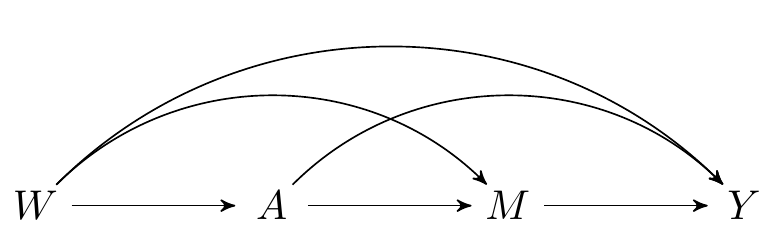
\includegraphics[width=0.8\linewidth]{01-preface_files/figure-latex/unnamed-chunk-2-1} 

}

\caption{Directed acyclic graph under *no intermediate confounders* of the mediator-outcome relation affected by treatment}\label{fig:unnamed-chunk-2}
\end{figure}

\hypertarget{intermediate-confounders}{%
\subsection{Intermediate confounders}\label{intermediate-confounders}}

\begin{figure}

{\centering \includegraphics[width=0.8\linewidth]{01-preface_files/figure-latex/unnamed-chunk-3-1} 

}

\caption{Directed acyclic graph under intermediate confounders of the mediator-outcome relation affected by treatment}\label{fig:unnamed-chunk-3}
\end{figure}

The above graphs can be interpreted as a \emph{non-parametric structural equation model}
(NPSEM), also known as \emph{structural causal model} (SCM):

\begin{align}
  W & = f_W(U_W)\\
  A & = f_A(W, U_A)\\
  Z & = f_Z(W, A, U_Z)\\
  M & = f_M(W, A, Z, U_M)\\
  Y & = f_Y(W, A, Z, M, U_Y)
\end{align}

\begin{itemize}
\tightlist
\item
  Here \(U=(U_W, U_A, U_Z, U_M, U_Y)\) is a vector of all unmeasured exogenous
  factors affecting the system
\item
  The functions \(f\) are assumed fixed but unknown
\item
  We posit this model as a system of equation that nature uses to geenrate the
  data at hand
\item
  Therefore we leave the functions \(f\) unspecified (i.e., we do not know the
  true nature mechanisms)
\item
  Sometimes we know something: e.g., if \(A\) is randomized we know \(A=f_A(U_A)\)
  where \(U_A\) is independent of everything.
\end{itemize}

\hypertarget{counterfactuals}{%
\section{Counterfactuals}\label{counterfactuals}}

\begin{itemize}
\tightlist
\item
  We define all the effects of interest using \emph{counterfactuals}
\item
  Counterfactuals are hypothetical random variables that would have been
  observed in a world where we would be able to perform interventions on the
  random variables of interest
\item
  \(Y_a\) is a counterfactual variable in a hypothetical world where \(\P(A=a)=1\)
  with probability one
\item
  \(Y_{a,m}\) is the counterfactual outcome in a world where \(\P(A=a,M=m)=1\)
\item
  \(M_a\) is the counterfactual variable representing the mediator in a world
  where \(\P(A=a)=1\).
\end{itemize}

\hypertarget{how-are-counterfactuals-defined}{%
\subsection{How are counterfactuals defined?}\label{how-are-counterfactuals-defined}}

\begin{itemize}
\tightlist
\item
  You can use counterfactual variables as \emph{primitives}
\item
  In the NPSEM framework, counterfactuals are quantities \emph{derived} from the
  model:
  \begin{align}
    Y_a  &= f_Y(W, a, Z, M, U_Y)\\
    Y_{a,m}  &= f_Y(W, a, Z, m, U_Y)\\
    M_a  &= f_M(W, a, Z, U_M)
  \end{align}
\item
  You can also define \emph{nested counterfactuals}
\item
  For example, if \(A\) is binary, you can think of the following counterfactual
  \begin{equation*}
    Y_{1, M_0} = f_Y(W, 1, Z, M_0, U_Y)
  \end{equation*}
\item
  Interpreted as \emph{the outcome for an individual in a hypothetical world where
  treatment was given but the mediator was held at the value it would have
  taken under no treatment}
\end{itemize}

\hypertarget{estimands}{%
\chapter{Path-specific casual mediation effect types}\label{estimands}}

\begin{itemize}
\tightlist
\item
  Controlled direct effects
\item
  Natural direct and indirect effects
\item
  Interventional direct and indirect effects
\end{itemize}

\begin{figure}

{\centering \includegraphics[width=0.8\linewidth]{02-effects-def_files/figure-latex/unnamed-chunk-1-1} 

}

\caption{Directed acyclic graph under *no intermediate confounders* of the mediator-outcome relation affected by treatment}\label{fig:unnamed-chunk-1}
\end{figure}

\hypertarget{controlled-direct-effects}{%
\section{Controlled direct effects}\label{controlled-direct-effects}}

\[\psi_{\text{CDE}} = \E(Y_{1,m} - Y_{0,m}) \]

\begin{itemize}
\tightlist
\item
  Set \(M=m\) uniformly for everyone in the population
\item
  Compare \(A=1\) vs \(A=0\) with \(M=m\) fixed
\end{itemize}

Under the below identification assumptions, the controlled direct can be identified:
\[ \E(Y_{1,m} - Y_{0,m}) = \E_w\{\E(Y \mid 1, m, w) - \E(Y \mid 0, m, w)\}\]

\hypertarget{identification-assumptions}{%
\subsection{Identification assumptions:}\label{identification-assumptions}}

\begin{itemize}
\tightlist
\item
  Confounder assumptions:

  \begin{itemize}
  \tightlist
  \item
    \(A \indep Y_{a,m} \mid W\)
  \item
    \(M \indep Y_{a,m} \mid W, A, Z\)
  \end{itemize}
\item
  Positivity assumptions:

  \begin{itemize}
  \tightlist
  \item
    \(\P(M = m \mid Z, A=a, W) > 0 \text{  } a.e.\)
  \item
    \(\P(A=a \mid W) > 0 \text{  } a.e.\)
  \end{itemize}
\end{itemize}

\begin{figure}

{\centering 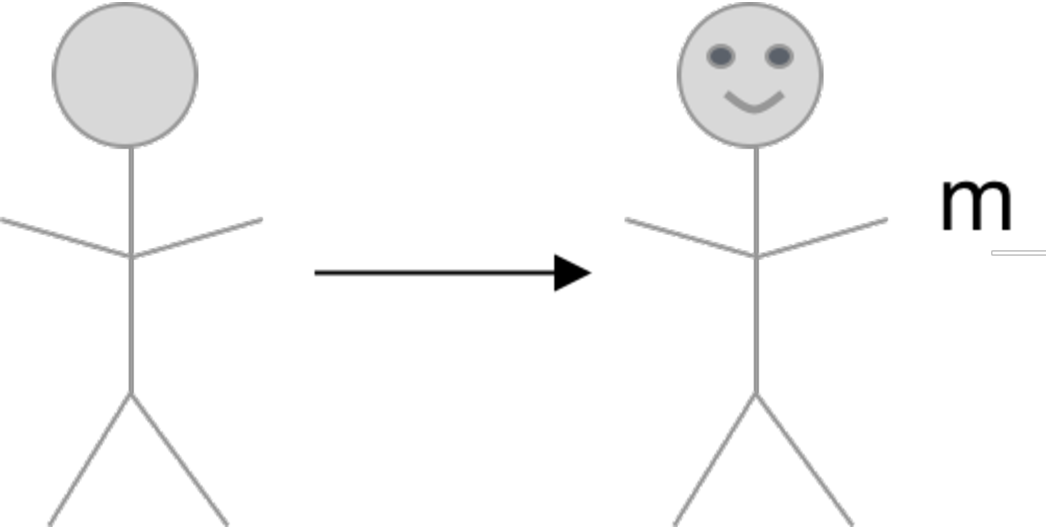
\includegraphics[width=0.5\linewidth]{/home/runner/work/ser2021_mediation_workshop/ser2021_mediation_workshop/img/graphic4a3} 

}

\end{figure}

\hypertarget{is-this-the-estimand-i-want}{%
\subsection{Is this the estimand I want?}\label{is-this-the-estimand-i-want}}

\begin{itemize}
\tightlist
\item
  Makes the most sense if can intervene directly on \(M\)

  \begin{itemize}
  \tightlist
  \item
    And can think of a policy that would set everyone to a single constant
    level \(m \in \mathcal{M}\).
  \item
    J. Pearl calls this \emph{prescriptive}.
  \item
    Can you think of an example?
  \item
    Air pollution, rescue inhaler dosage, hospital visits
  \item
    Does not provide a decomposition of the average treatment effect into direct and indirect effects
  \end{itemize}
\end{itemize}

\emph{What if our research question doesn't involve intervening directly on the
mediator?}

\emph{What if we want to decompose the average treatment effect into its direct and
indirect counterparts?}

\hypertarget{natural-direct-and-indirect-effects}{%
\section{Natural direct and indirect effects}\label{natural-direct-and-indirect-effects}}

Still using the same DAG as above,

Natural direct effect (NDE):
\begin{equation*}
  \psi_{\text{NDE}} = \E(Y_{1,M_0} - Y_{0,M_0})
\end{equation*}

Natural indirect effect (NIE):
\begin{equation*}
  \psi_{\text{NIE}} = \E(Y_{1,M_1} - Y_{1,M_0})
\end{equation*}

If the cross-world assumption holds (defined below), the NDE can also be written
as: \(\E_W \sum_m \{\E(Y_{1,m} \mid W) - \E(Y_{0,m} \mid W)\} \P(M_{0}=m \mid W)\)

\begin{itemize}
\tightlist
\item
  Weighted average of controlled direct effects at each level of \(m\).
\item
  If no effect modification of the effect of \(A\) on \(Y\) by \(M\) (i.e., no interaction between \(A\) and \(M\)), then CDE = NDE.
\end{itemize}

\begin{figure}

{\centering 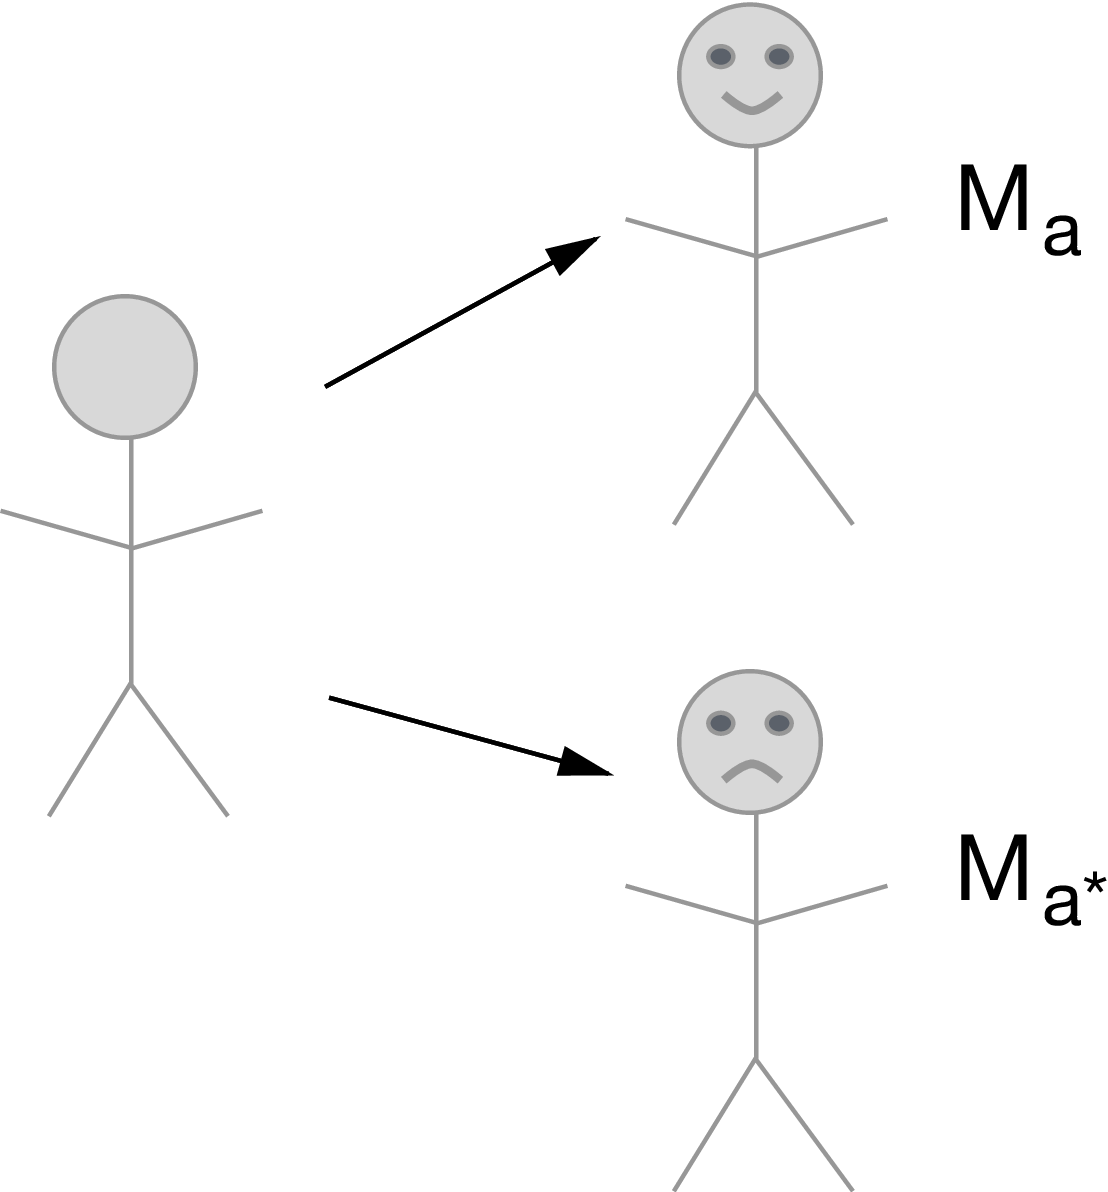
\includegraphics[width=0.5\linewidth]{/home/runner/work/ser2021_mediation_workshop/ser2021_mediation_workshop/img/graphic4a} 

}

\end{figure}

Under the below identification assumptions, the natural direct effect can be identified:
\begin{equation*}
\E(Y_{1,M_0} - Y_{0,M_0}) =
  \E_w\{\sum_m \{\E(Y \mid 1, m, w) - \E(Y \mid 0, m, w)\} P(M=m \mid A=0,w)\}
\end{equation*}
(The natural indirect effect can be identified similarly.)

\hypertarget{identification-assumptions-1}{%
\subsection{Identification assumptions:}\label{identification-assumptions-1}}

\begin{itemize}
\tightlist
\item
  \(A \indep Y_{a,m} \mid W\)
\item
  \(M \indep Y_{a,m} \mid W, A\)
\item
  \(A \indep M_a \mid W\)
\item
  \(M_0 \indep Y_{1,m} \mid W\)
\item
  and positivity assumptions
\end{itemize}

What does \(M_0 \indep Y_{1,m} \mid W\) mean?

\begin{itemize}
\tightlist
\item
  Conditional on \(W\), knowledge of \(M\) in the absence of treatment \(A\)
  provides no information of the effect of \(A\) on \(Y\).
\item
  Can you think of a data-generating mechanism that would violate this
  assumption?
\item
  Whenever we believe that treatment assignment works through adherence (i.e., almost
  always), we are violating this assumption.
\end{itemize}

\hypertarget{is-this-the-estimand-i-want-1}{%
\subsection{Is this the estimand I want?}\label{is-this-the-estimand-i-want-1}}

\begin{itemize}
\tightlist
\item
  Makes sense to intervene on \(A\) but not directly on \(M\).
\item
  Want to understand a natural mechanism underlying an association/ total
  effect. J. Pearl calls this \emph{descriptive}.
\item
  NDE + NIE = total effect (ATE).
\item
  Okay with the assumptions.
\end{itemize}

\emph{What if our data structure involves a post-treatment confounder of the
mediator-outcome relationship (e.g., adherence)?}

\begin{figure}

{\centering \includegraphics[width=0.8\linewidth]{02-effects-def_files/figure-latex/unnamed-chunk-3-1} 

}

\caption{Directed acyclic graph under intermediate confounders of the mediator-outcome relation affected by treatment}\label{fig:unnamed-chunk-3}
\end{figure}

\begin{figure}

{\centering 
\includegraphics[width=1\linewidth]{/home/runner/work/ser2021_mediation_workshop/ser2021_mediation_workshop/img/ctndag} 

}

\end{figure}

\hypertarget{unidentifiability-of-the-nde-and-nie-in-this-setting}{%
\subsection{Unidentifiability of the NDE and NIE in this setting}\label{unidentifiability-of-the-nde-and-nie-in-this-setting}}

In this example, natural direct and indirect effects are
unidentifiable from observed data on \((W,A,Z,M,Y)\). The technical
reason for this is that the cross-world counterfactual assumption
\begin{equation*}
  Y(1,m)\indep M(0)\mid W
\end{equation*}

does not hold in the above directed acyiclic graph. Intuitively, the
reason for this is that an intervention setting \(A=1\) (necessary for
the definition of \(Y(1,m)\)) induces a counterfactual variable
\(Z(1)\). Likewise, an intervention setting \(A=0\) (necessary for the
definition of \(M(0)\)) induces a counterfactual \(Z(0)\). The variables
\(Z(1)\) and \(Z(0)\) are correlated because they share unmeasured common
causes. The variable \(Z(1)\) is correlated with \(Y(1,m)\), and the
variable \(Z(0)\) is correlated with \(M(0)\), because they are
counterfactual outcomes in the same hypothetical worlds. Thus, to
achieve \(Y(1,m)\) independent of \(M(0)\), it would be necessary to
adjust for either \(Z(1)\) or \(Z(0)\). This is impossible to do since
these variables are unmeasured.

Note: CDEs are still identified in this setting. They can be estimated similarly to two-time-point intervention.

\hypertarget{interventional-indirect-effects}{%
\section{Interventional (in)direct effects}\label{interventional-indirect-effects}}

\begin{itemize}
\item
  Let \(G_{M \mid a, W}\) denote a random draw from the distribution of \(M(a) \mid W\)
\item
  Define the counterfactual \(Y(1,G_{M \mid 0, W})\) as the counterfactual
  variable in a hypothetical world where \(A\) is set \(A=1\) and \(M\) is
  set to \(M=G_{M \mid 0, W}\) with porbability one.
\item
  Define \(Y(0,G_{M \mid 0, W})\) and \(Y(1,G_{M \mid 1, W})\) similarly
\item
  Then we can define:
  \begin{equation*}
    \E[Y(1,G_{M \mid 1, W}) - Y(0,G_{M \mid 0, W})] = \underbrace{\E[Y(1,G_{M \mid 1, W}) -
      Y(1,G_{M \mid 0, W})]}_{\text{interventional indirect effect}} +
      \underbrace{\E[Y(1,G_{M \mid 0, W}) -
      Y(0,G_{M \mid 0, W})]}_{\text{interventional direct effect}}
  \end{equation*}
\item
  Note that \(G_{M \mid a^{\star}, W}\) represents a
  stochastic intervention on the mediator, where value \(m\) is drawn with
  probability \(\P(M = m \mid A = a^{\star}, W = w)\)
\item
  Marginal PIDE: \(\E(Y_{a, g_{M \mid a^{\star}, W}}) - \E(Y_{a^{\star}, g_{M \mid a^{\star}, W}})\)
\item
  Marginal PIIE: \(\E(Y_{a, g_{M \mid a, W}}) - \E(Y_{a, g_{M \mid a^{\star}, W}})\)
\item
  Conditional PIDE: \(\E(Y_{a, g_{M \mid Z, a^{\star}, W}}) - \E(Y_{a^{\star}, g_{M \mid Z, a^{\star}, W}})\)
\item
  Conditional PIIE: \(\E(Y_{a, g_{M \mid Z, a, W}}) - \E(Y_{a, g_{M \mid Z, a^{\star}, W}})\)
\item
  Can you think of an example when you would want the conditional versions?
  Marginal versions?
\end{itemize}

\begin{figure}

{\centering 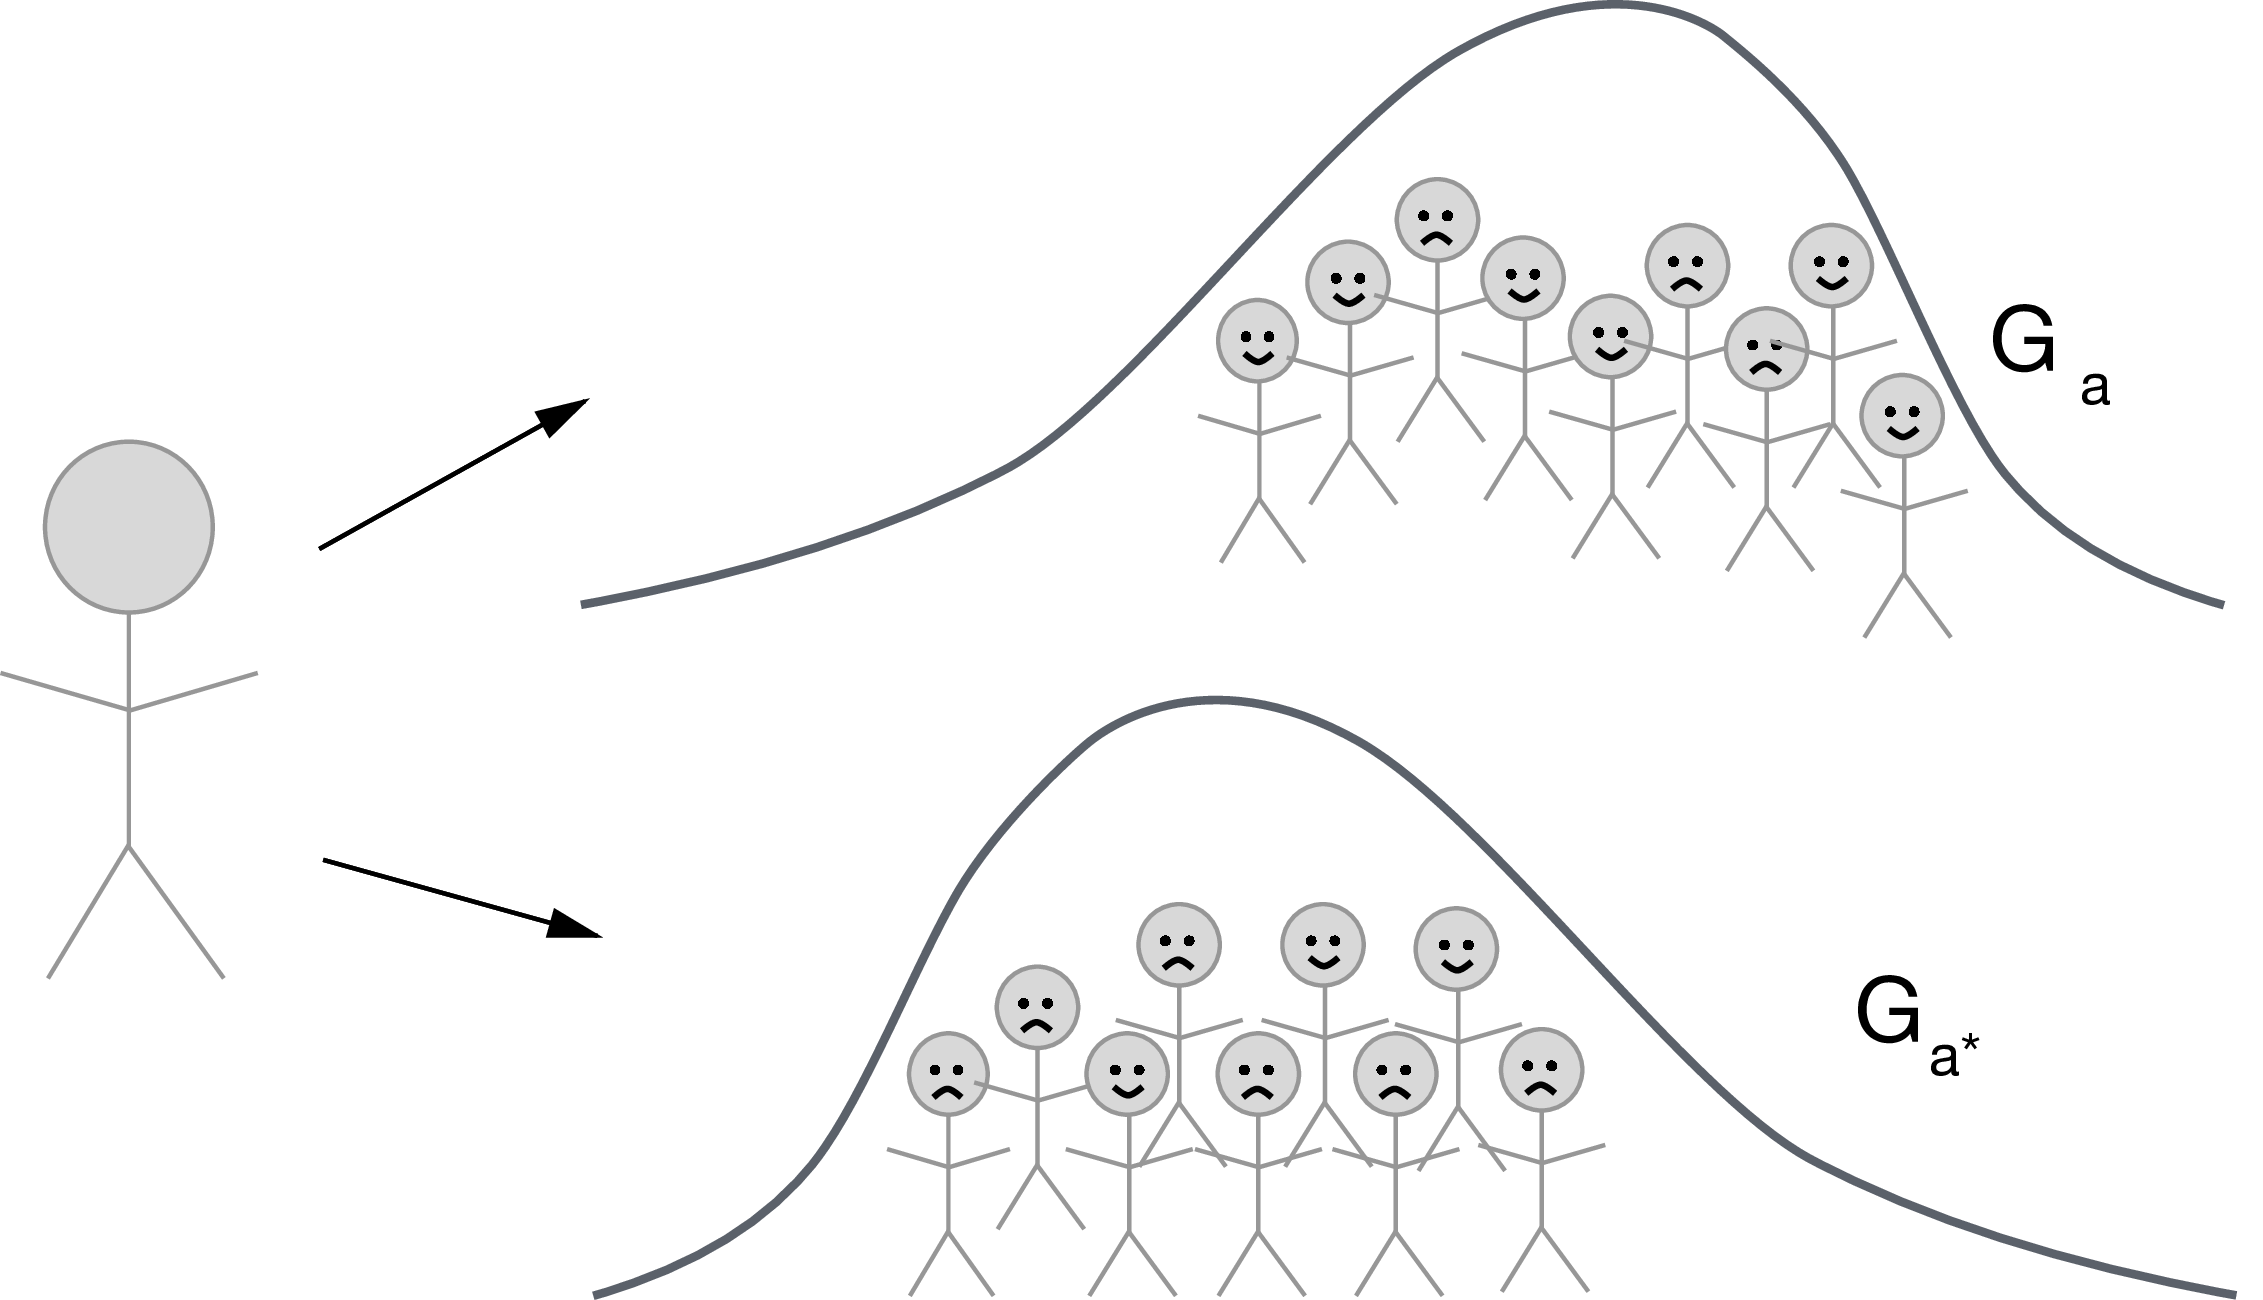
\includegraphics[width=0.5\linewidth]{/home/runner/work/ser2021_mediation_workshop/ser2021_mediation_workshop/img/graphic4b} 

}

\end{figure}

Under the following identification assumptions, the population interventional direct effect is identified:
\begin{equation*}
\E(Y_{1, g_{M \mid 0, W}}) - \E(Y_{0, g_{M \mid 0, W}}) = \E_w \{\sum_{z,m}
  \{\E(Y \mid 1, z, m, w) P(z \mid 1, w) - \E(Y \mid 1, z, m, w)
  P(z \mid 0, w)\} P(m \mid A=0, w) \}
\end{equation*}

\hypertarget{identification-assumptions-2}{%
\subsection{Identification assumptions:}\label{identification-assumptions-2}}

\begin{itemize}
\tightlist
\item
  \(A \indep Y_{a,m} \mid W\)
\item
  \(M \indep Y_{a,m} \mid W, A\)
\item
  \(A \indep M_a \mid W\)
\item
  and positivity assumptions.
\end{itemize}

Is this the estimand I want?

\begin{itemize}
\tightlist
\item
  Makes sense to intervene on \(A\) but not directly on \(M\).
\item
  Goal is to understand a natural mechanism underlying an association or total
  effect.
\item
  Okay with the assumptions!
\end{itemize}

\hypertarget{estimand-summary}{%
\section{Estimand Summary}\label{estimand-summary}}

\begin{figure}

{\centering 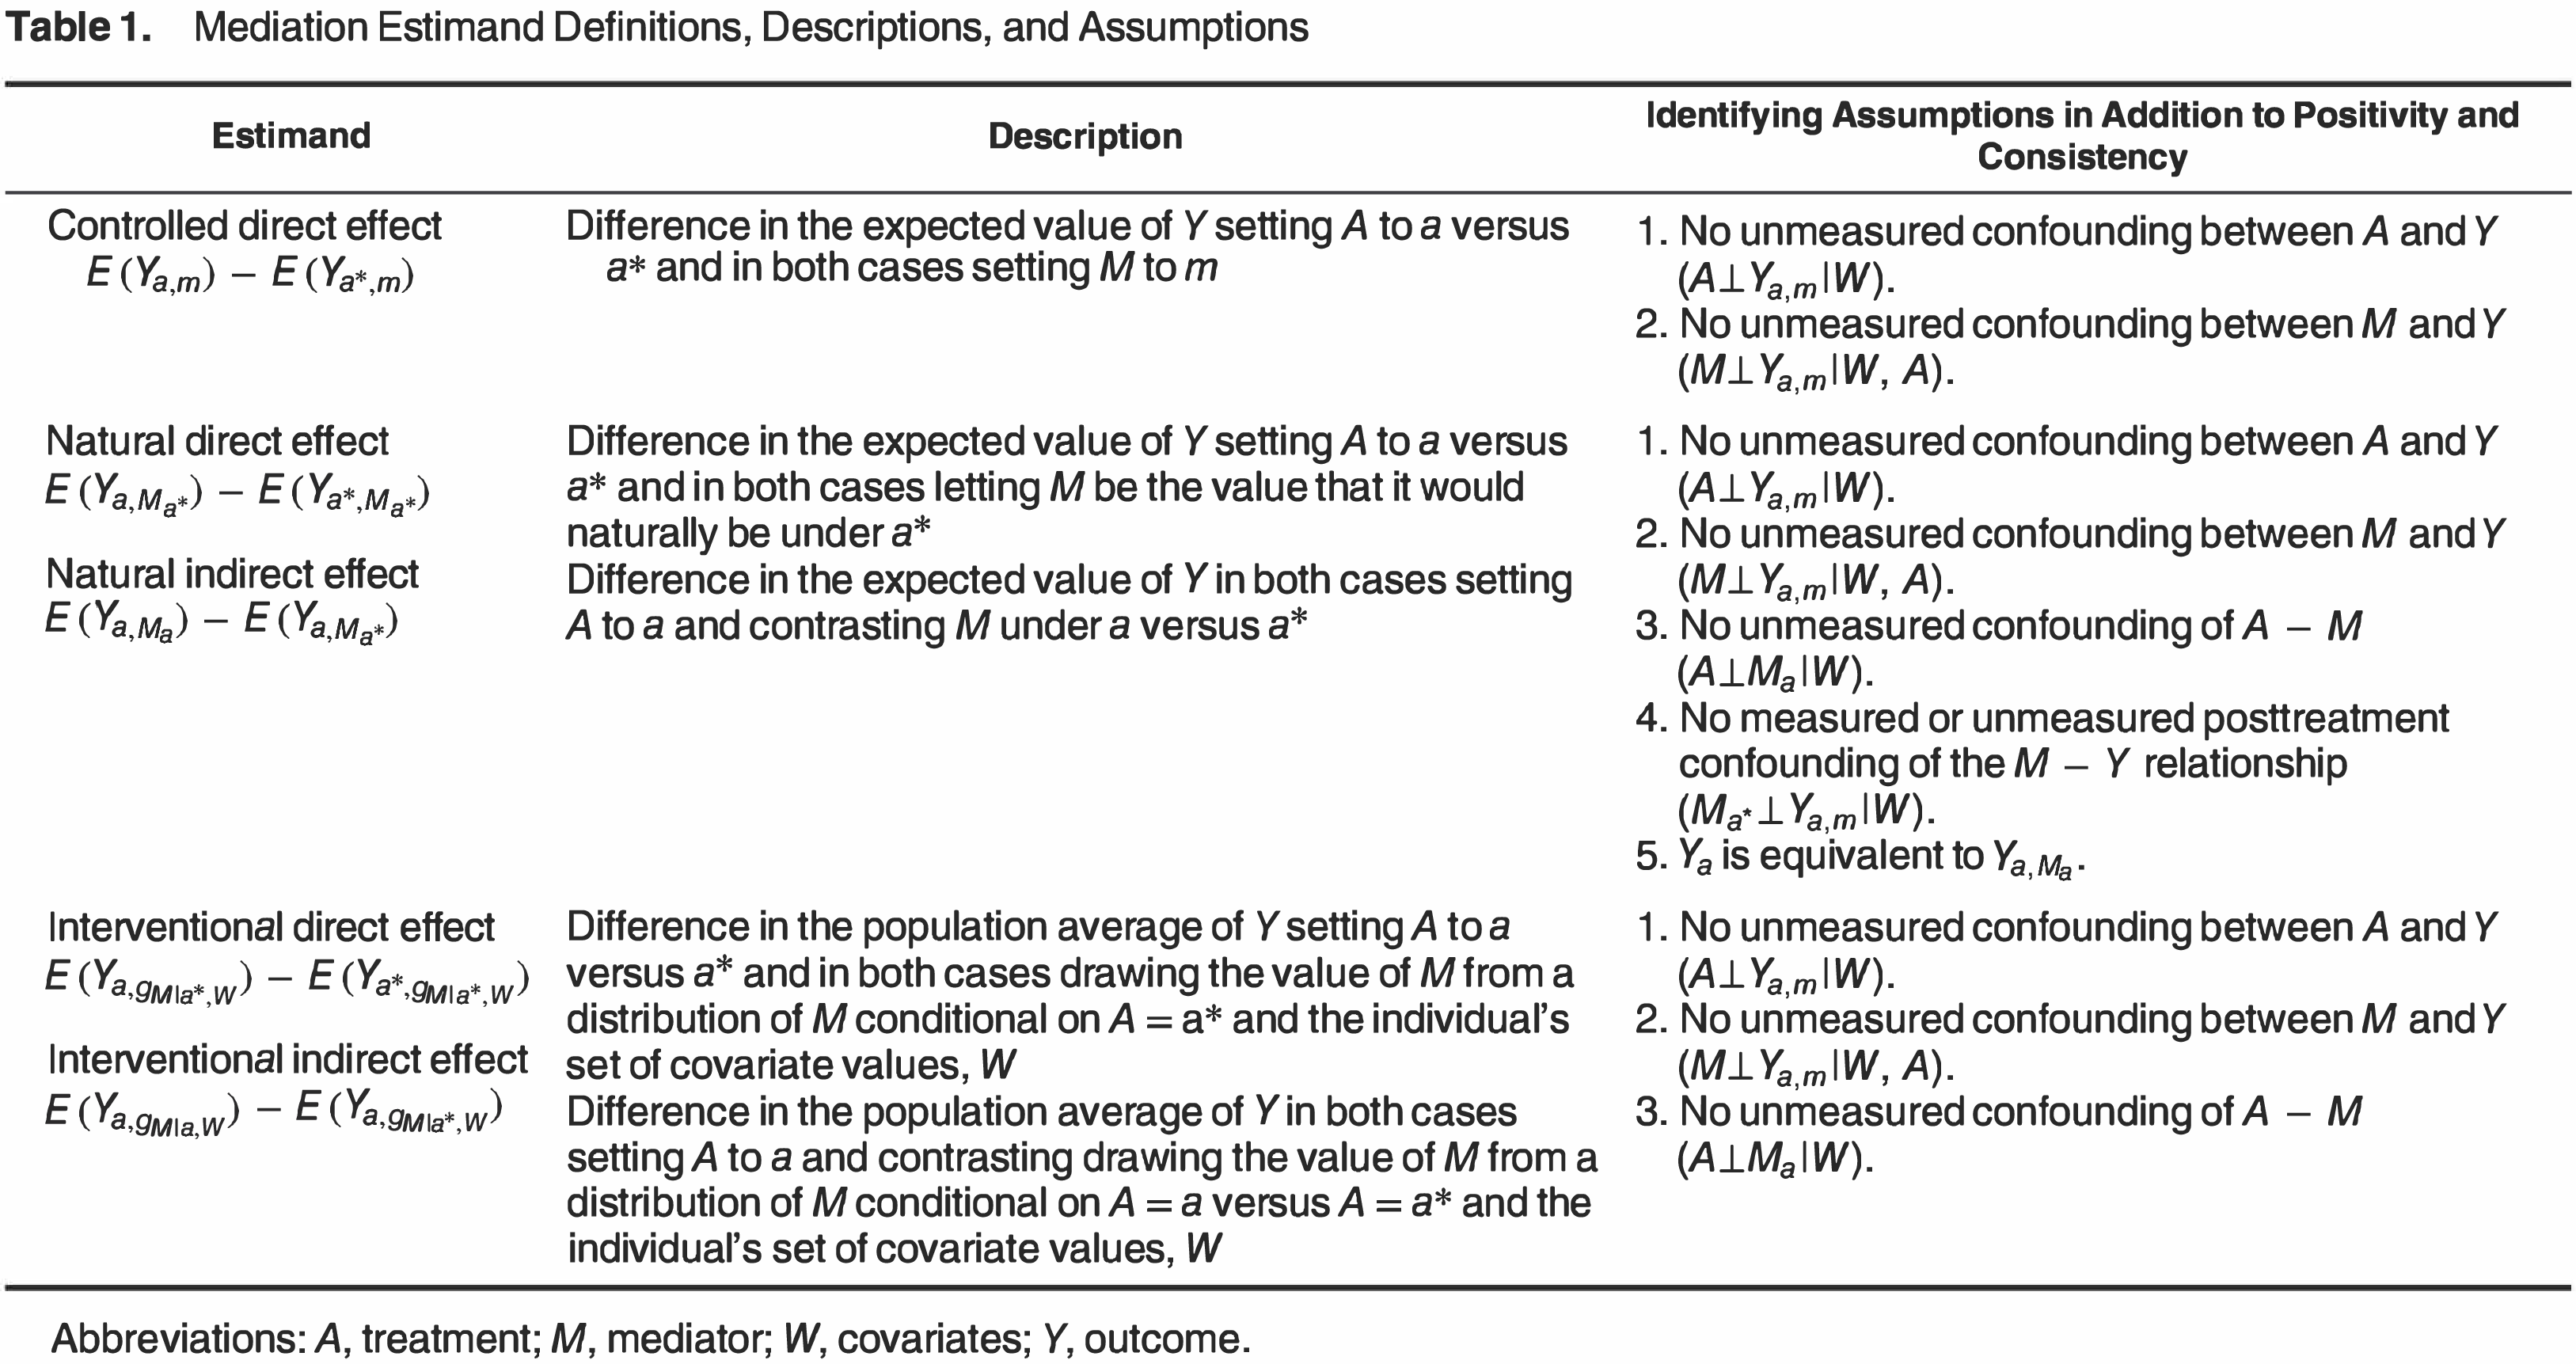
\includegraphics[width=1.25\linewidth]{/home/runner/work/ser2021_mediation_workshop/ser2021_mediation_workshop/img/table1} 

}

\end{figure}

\hypertarget{estimandirl}{%
\chapter{How to choose an estimand: Real world example}\label{estimandirl}}

\hypertarget{comparative-effectivness-of-two-medications-for-opioid-use-disorder-oud}{%
\section{Comparative effectivness of two medications for opioid use disorder (OUD)}\label{comparative-effectivness-of-two-medications-for-opioid-use-disorder-oud}}

\begin{figure}

{\centering 
\includegraphics[width=1\linewidth]{/home/runner/work/ser2021_mediation_workshop/ser2021_mediation_workshop/img/ctndag} 

}

\end{figure}

\emph{Motivation}: Opposite overall treatment effects for homeless versus
nonhomeless participants.

\begin{figure}

{\centering 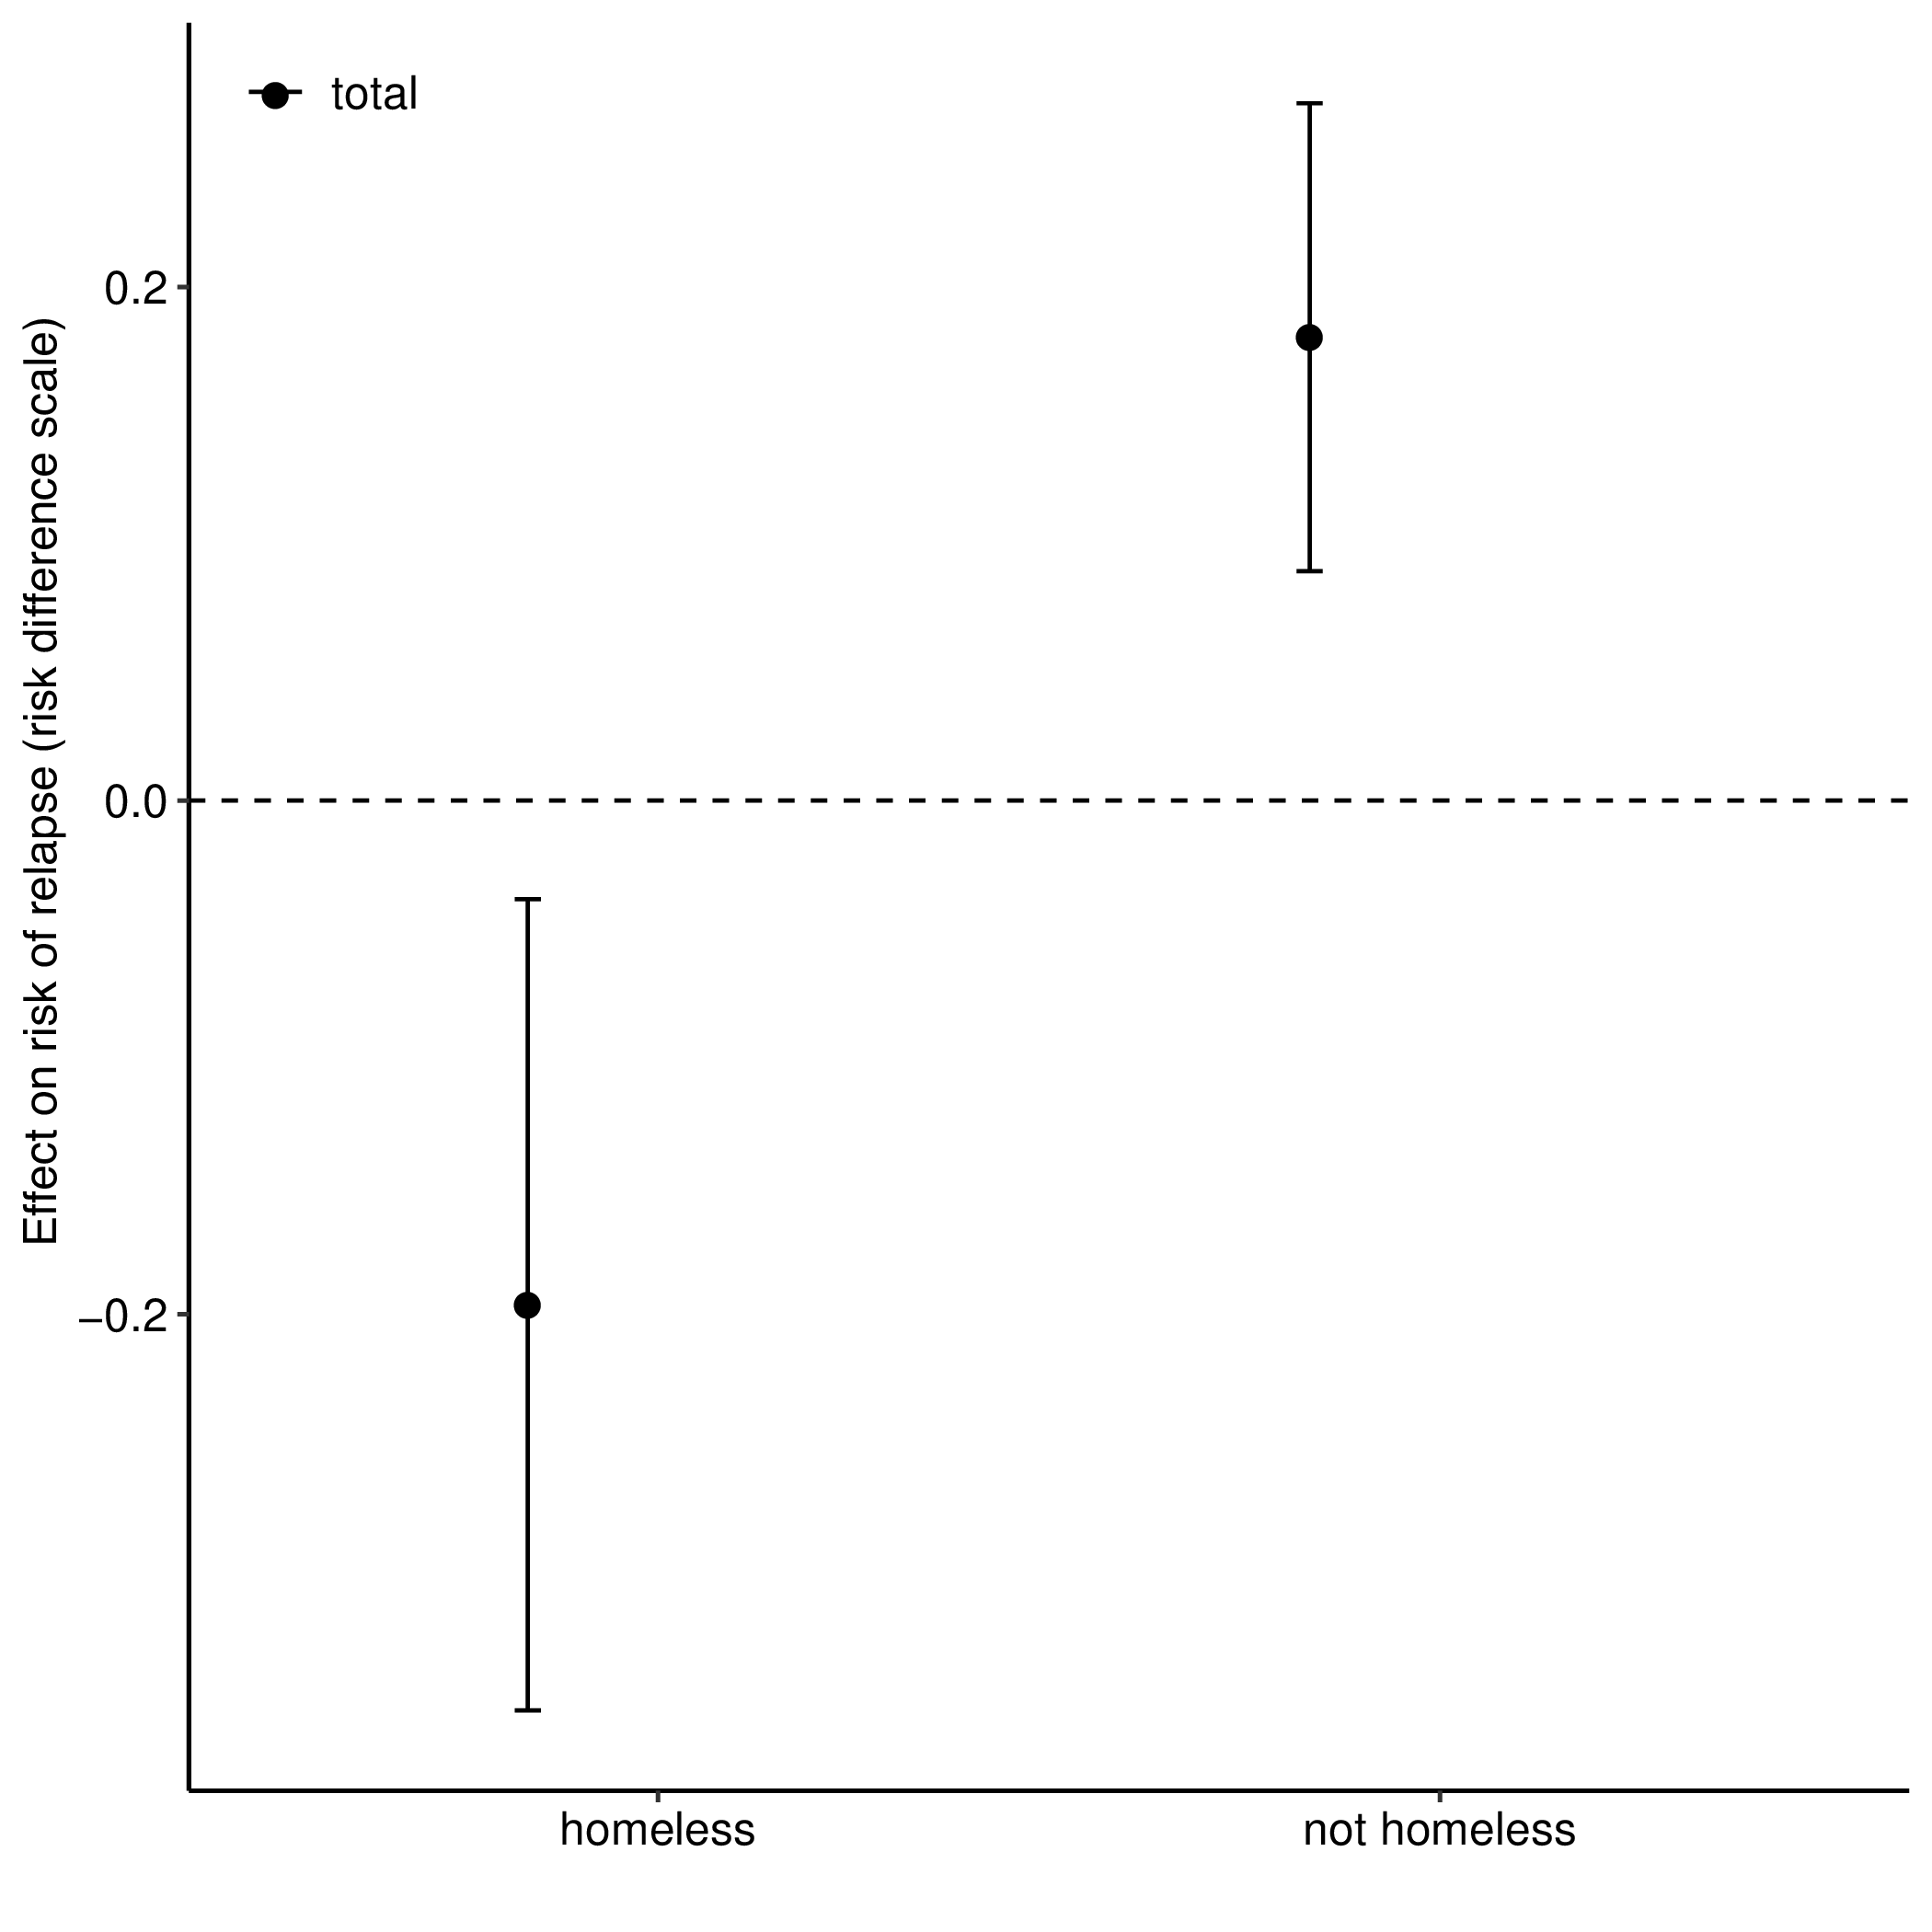
\includegraphics[width=0.5\linewidth]{/home/runner/work/ser2021_mediation_workshop/ser2021_mediation_workshop/img/tmleesttotal} 

}

\end{figure}

\hypertarget{getting-specific-about-the-question}{%
\subsection{Getting specific about the question}\label{getting-specific-about-the-question}}

To what extent does the indirect effect through mediators of adherence, pain, and
depressive symptoms explain the differences in treatment effects on OUD relapse
for homeless and nonhomeless individuals?

What estimand do we want?

\begin{itemize}
\tightlist
\item
  Can we set \(M=m\) (i.e., same value) for everyone?
\item
  Are we interested in estimating indirect effects?
\end{itemize}

\(\rightarrow\) So, \emph{not} controlled direct effect.

\begin{itemize}
\tightlist
\item
  Do we have an intermediate confounder?
\item
  Yes, and it's important.
\end{itemize}

\(\rightarrow\) So, \emph{not} natural (in)direct effects.

\begin{itemize}
\tightlist
\item
  So, we're left with the interventional direct and indirect effects.
\item
  Do we want to estimate the path through treatment initiation (\(Z\))?
\item
  Yes, so, \emph{not} the conditional versions of these effects.
\item
  Estimands:

  \begin{itemize}
  \tightlist
  \item
    Direct effect: \(\E(Y_{1,g_0} - Y_{0,g_0})\)
  \item
    Indirect effect: \(\E(Y_{1,g_1} - Y_{1,g_0})\)
  \end{itemize}
\item
  Need to incorporate multiple and continuous mediators
\end{itemize}

\hypertarget{stochastic}{%
\chapter{Stochastic Direct and Indirect Effects}\label{stochastic}}

\hypertarget{definition-of-the-effects}{%
\section{Definition of the effects}\label{definition-of-the-effects}}

Consider the following directed acyclic graph.

\begin{figure}

{\centering \includegraphics[width=0.8\linewidth]{04-stochastic_files/figure-latex/unnamed-chunk-1-1} 

}

\caption{Directed acyclic graph under no intermediate confounders of the mediator-outcome relation affected by treatment}\label{fig:unnamed-chunk-1}
\end{figure}

\hypertarget{motivation-for-stochastic-interventions}{%
\section{Motivation for stochastic interventions}\label{motivation-for-stochastic-interventions}}

\begin{itemize}
\tightlist
\item
  So far we have discussed controlled, natural, and interventional (in)direct effects
\item
  These effects require that \(0 < \P(A=1\mid W) < 1\)
\item
  They are defined only for binary exposures
\item
  \emph{What can we do when the positivity assumption does not hold or the exposure
  is continuous?}
\item
  Solution: we can use stochastic effects
\end{itemize}

\hypertarget{definition-of-stochastic-effects}{%
\section{Definition of stochastic effects}\label{definition-of-stochastic-effects}}

There are two possible ways of defining stochastic effects:

\begin{itemize}
\tightlist
\item
  Consider the effect of an intervention where the exposure is drawn from a
  distribution

  \begin{itemize}
  \tightlist
  \item
    Example: {[}TO FILL IN{]}
  \end{itemize}
\item
  Consider the effect of an intervention where the post-intervention exposure is
  a function of the actually received exposure

  \begin{itemize}
  \tightlist
  \item
    Example: {[}TO FILL IN{]}
  \end{itemize}
\item
  In both cases \(A\mid W\) is non-deterministic, thus the name \emph{stochastic intervention}
\end{itemize}

\hypertarget{example-incremental-propensity-score-interventions-ipsi-kennedy2018nonparametric}{%
\subsection*{\texorpdfstring{Example: incremental propensity score interventions (IPSI) \citep{kennedy2018nonparametric}}{Example: incremental propensity score interventions (IPSI) {[}@kennedy2018nonparametric{]}}}\label{example-incremental-propensity-score-interventions-ipsi-kennedy2018nonparametric}}


\hypertarget{definition-of-the-intervention}{%
\subsubsection*{Definition of the intervention}\label{definition-of-the-intervention}}


\begin{itemize}
\tightlist
\item
  Assume \(A\) is binary, and \(\P(A=1\mid W=w) = g(1\mid w)\) is the propensity score
\item
  Consider an intervention in which each individual receives the intervention
  with probability \(g_\delta(1\mid w)\), equal to
  \begin{equation*}
    g_\delta(1\mid w)=\frac{\delta g(1\mid w)}{\delta g(1\mid w) +
    1 - g(1\mid w)}
  \end{equation*}
\item
  e.g., draw the post-intervention exposure from a Bernoulli variable with
  probability \(g_\delta(1\mid w)\)
\item
  The value \(\delta\) is user given
\item
  Let \(A_\delta\) denote the post-intervention distribution
\item
  Some algebra shows that \(\delta\) is an odds ratio comparing the pre- and
  post-intervantion distributions
  \begin{equation*}
    \delta = \frac{\text{odds}(A_\delta = 1\mid W=w)}
    {\text{odds}(A = 1\mid W=w)}
  \end{equation*}
\item
  This gives the intervention a nice interpretation as \emph{what would happen in a
  world where the odds of receiving treatment is increased by \(\delta\)}
\item
  Let \(Y_{A_\delta}\) denote the outcome in this hypothetical world
\end{itemize}

\hypertarget{example-modified-treatment-policies}{%
\subsection{Example: modified treatment policies}\label{example-modified-treatment-policies}}

\hypertarget{definition-of-the-intervention-1}{%
\subsubsection*{Definition of the intervention}\label{definition-of-the-intervention-1}}


\hypertarget{mediation-analysis-for-stochastic-interventions}{%
\subsection{Mediation analysis for stochastic interventions}\label{mediation-analysis-for-stochastic-interventions}}

\begin{itemize}
\tightlist
\item
  The total effect of an IPSI can be computed as a contrast of the outcome under
  intervention vs no intervention:
  \begin{equation*}
    \psi = \E[Y_{A_\delta} - Y]
  \end{equation*}
\item
  Recall the NPSEM
  \begin{align}
    W & = f_W(U_W)\\
    A & = f_A(W, U_A)\\
    M & = f_M(W, A, U_M)\\
    Y & = f_Y(W, A, M, U_Y)
  \end{align}
\item
  From this we have \(Y_{A_\delta} = f_Y(W, A_\delta, M_{A_\delta}, U_Y)\)
\item
  Thus, we have \(Y_{A_\delta} = Y_{A_\delta, M_{A_\delta}}\) and \(Y = Y(A,M(A))\)
\item
  Let us introduce the counterfactual \(Y_{A_\delta,M}\), interpreted as the
  outcome observed in a world where the intervention on \(A\) is performed but the
  mediator is fixed at the value it would have taken under no intervention
\item
  Then we can decompose the total effect into:
  \begin{align*}
    \E[Y&_{A_\delta,M_{A_\delta}} - Y_{A,M_A}] = \\
    &\underbrace{\E[Y_{A_\delta,M_{A_\delta}} -
      Y_{A_\delta,M_A}]}_{\text{stochastic natural indirect effect}} +
      \underbrace{\E[Y_{A,M_{A_\delta}} -
      Y_{A,M_A}]}_{\text{stochastic natural direct effect}}
  \end{align*}
\end{itemize}

\hypertarget{identification-of-the-effect-of-a-stochastic-intervention}{%
\section{Identification of the effect of a stochastic intervention}\label{identification-of-the-effect-of-a-stochastic-intervention}}

\hypertarget{preliminaries-on-semiparametric-estimation}{%
\chapter{Preliminaries on semiparametric estimation}\label{preliminaries-on-semiparametric-estimation}}

\hypertarget{why-do-we-need-new-estimation-tools}{%
\section{Why do we need new estimation tools?}\label{why-do-we-need-new-estimation-tools}}

\begin{itemize}
\item
  As we have seen all the mediation parameters that we consider can be
  seen as a function of the joint probability distribution of \(O=(W,A,Z,M,Y)\)
\item
  For example, under identifiability assumptions the natural direct effect is
  equal to
  \begin{equation*}
    \psi(\P) =  \sum_{m,w}\big[\E(Y\mid A=1,M=m,W=w) -
      \E(Y\mid A=0,M=m,W=w)\big]\P(M=m\mid A=0, W=w)\P(W=w)
  \end{equation*}
\item
  The notation \(\psi(\P)\) implies that the parameter is a function of \(\P\)
\item
  This means that we can compute it for any distribution \(\P\)
\item
  For example, if we know the true \(\P(W,A,M,Y)\), we can comnpute the true value
  of the parameter by:

  \begin{itemize}
  \tightlist
  \item
    Computing the conditional expectation \(\E(Y\mid A=1,M=m,W=w)\) for all values
    \((m,w)\)
  \item
    Computing the probability \(\P(M=m\mid A=0,W=w)\) for all values \((m,w)\)
  \item
    Computing the probability \(\P(W=w)\) for all values \(w\)
  \item
    Computing the sum over all values \((m,w)\)
  \end{itemize}
\item
  This is how you would compute the \emph{true value} \textbf{if you knew} the true
  distribution \(\P\)
\item
  But we can use the same logic for estimation:

  \begin{itemize}
  \tightlist
  \item
    Fit a regression to estimate \(\E(Y\mid A=1,M=m,W=w)\)
  \item
    Fit a regression to estimate \(\P(M=m\mid A=0,W=w)\)
  \item
    Estimate \(\P(W=w)\) with the empirical distribution
  \end{itemize}
\item
  This is known as the g-computation estimator (more on this estimator later)
\end{itemize}

\hypertarget{how-can-g-estimation-be-implemented-in-practice}{%
\subsection{How can g-estimation be implemented in practice?}\label{how-can-g-estimation-be-implemented-in-practice}}

\begin{itemize}
\tightlist
\item
  There are two possible ways to do g-computation estimation:

  \begin{itemize}
  \tightlist
  \item
    Using parametric models for the above regressions
  \item
    Using flexible data-adaptive regression (aka machine learning)
  \end{itemize}
\end{itemize}

\hypertarget{pros-and-cons-of-parametric-models}{%
\subsection{Pros and cons of parametric models}\label{pros-and-cons-of-parametric-models}}

\begin{itemize}
\tightlist
\item
  Pros:

  \begin{itemize}
  \tightlist
  \item
    Easy to understand
  \item
    Ease of implementation (standard regression software)
  \item
    Can use the Delta method or the bootstrap for computation of standard errors
  \end{itemize}
\item
  Cons:

  \begin{itemize}
  \tightlist
  \item
    Unless \(W\) and \(M\) contain very few categorical variables, it is very easy
    to misspecify the models
  \item
    This can introduce sizable bias in the estimators
  \item
    This bias is highly problematic

    \begin{itemize}
    \tightlist
    \item
      We go through a thorough process to correctly specify our causal models to
      avoid bias
    \item
      Overly simplisitc models introduce bias and squander those efforts
    \item
      The bias can be small or large and you can never know from a single data
      analysis
    \end{itemize}
  \end{itemize}
\end{itemize}

\hypertarget{pros-and-cons-of-g-computation-with-data-adaptive-regression}{%
\subsection{Pros and cons of g-computation with data-adaptive regression}\label{pros-and-cons-of-g-computation-with-data-adaptive-regression}}

\begin{itemize}
\tightlist
\item
  Pros:

  \begin{itemize}
  \tightlist
  \item
    Easy to understand
  \item
    Alleviate model-misspecification bias
  \end{itemize}
\item
  Cons:

  \begin{itemize}
  \tightlist
  \item
    Might be harder to implement depending on the regression procedure
  \item
    No general approaches for computation of standard errors and confidence
    intervals
  \end{itemize}
\end{itemize}

\hypertarget{semiparametric-estimation---an-alternative-to-solve-these-problems}{%
\section{Semiparametric estimation - an alternative to solve these problems}\label{semiparametric-estimation---an-alternative-to-solve-these-problems}}

\hypertarget{biasvariance-tradeoff}{%
\subsection{Bias/variance tradeoff}\label{biasvariance-tradeoff}}

\begin{itemize}
\item
  A lot of the recent literature in causal inference with data-adaptive
  regression uses the following ideas
\item
  G-computation estimation with data-adaptive regression offers an incorrect
  bias/variance trade-off
\item
  Specifically, the bias of a g-computation estimator can often be expressed as
  \begin{equation*}
    \psi(\hat\P) - \psi(\P) \approx -\E[D(O;\hat\P)]
  \end{equation*}
\item
  The function \(D(O;\P)\) is called \emph{the efficient influence function} (EIF)
\item
  The EIF must be found on a case-by-case basis or each parameter \(\psi(\P)\)
\item
  For example, for estimating the standardized mean \(\psi(P)=\E[\E(Y\mid A=1, W)]\), we have
  \begin{equation*}
    D(O,\hat\P) = \frac{A}{\hat P(A=1\mid W)}[Y - \hat\E(Y\mid A=1, W)] +
    \hat\E(Y\mid A=1, W) - \psi(\hat\P)
  \end{equation*}
\item
  In this workshop we will not present the specific form of \(D(O;\hat\P)\) for
  all parameters that we use
\item
  But the estimators we discuss and implement in the packages will be based on
  theser EIFs
\end{itemize}

\hypertarget{bias-correction-of-g-computation-estimators}{%
\subsection{Bias-correction of g-computation estimators}\label{bias-correction-of-g-computation-estimators}}

\begin{itemize}
\tightlist
\item
  There are at least two ways to use the EIF to perform a bias correction for a
  g-computation estimator
\item
  The first one is the so-called \emph{one step} estimator:
  \begin{equation*}
    \psi(\hat \P) + \frac{1}{n}\sum_{i=1}^n D(O;\hat \P_i)
  \end{equation*}
\item
  The idea behind the one-step estimator is simple: subtract an estimate of the
  bias of the g-computation estimator
\item
  The second approach is the \emph{targeted maximum likelihood estimator} (TMLE)
\item
  TMLE is based on the principle that it is possile to construct a
  data-adaptive estimator \(\tilde \P\) such that
  \begin{equation*}
    \frac{1}{n}\sum_{i=1}^n D(O;\tilde \P_i)=0
  \end{equation*}
\item
  Thus, for this special data-adaptive estimate \(\tilde \P\), the TMLE is
  actually just the g-computation estimator \(\psi(\tilde\P)\)
\end{itemize}

\hypertarget{estimating-natural-and-interventional-effects}{%
\chapter{Estimating natural and interventional effects}\label{estimating-natural-and-interventional-effects}}

\hypertarget{natural-indirect-effects}{%
\section{Natural (in)direct effects}\label{natural-indirect-effects}}

Recall:

\begin{figure}

{\centering \includegraphics[width=0.8\linewidth]{06-estimation-natural-interventional_files/figure-latex/unnamed-chunk-1-1} 

}

\caption{Directed acyclic graph under *no intermediate confounders* of the mediator-outcome relation affected by treatment}\label{fig:unnamed-chunk-1}
\end{figure}

Assuming a binary \(A\), we define the natural direct effect as:
\[NDE = E(Y_{1,M_{0}} - Y_{0,M_{0}})\],

and the natural indirect effect as:
\[NIE = E(Y_{1,M_{1}} - Y_{1,M_{0}})\].

\hypertarget{simple-case-for-intuition}{%
\subsection{Simple case for intuition}\label{simple-case-for-intuition}}

The observed data is \(O=(W, A, M, Y)\)

This SCM is represented in the above DAG and the following causal models:
\begin{align*}
  W & = f_W(U_W)\\
  A & = f_A(W, U_A)\\
  M & = f_M(W, A, U_M)\\
  Y & = f_Y(W, A, M, U_Y),
\end{align*}
where \((U_W, U_A,U_M, U_Y)\) are exogenous random errors.

We assume
- \(A\) is a single binary randomized treatment (and thus \(A = f_A(U_A)\))
- \(M\) is a single binary mediator
- There are no restrictions on the distribution of \(W\) or \(Y\)

Recall that we need to assume the following to identify the above caual effects
from our observed data:

\begin{itemize}
\tightlist
\item
  \(A \indep Y_{a,m} \mid W\)
\item
  \(M \indep Y_{a,m} \mid W, A\)
\item
  \(A \indep M_a \mid W\)
\item
  \(M_0 \indep Y_{1,m} \mid W\)
\item
  and positivity assumptions
\end{itemize}

\hypertarget{how-to-estimate-using-g-computation}{%
\subsection{How to estimate using G-computation}\label{how-to-estimate-using-g-computation}}

Let's take the NDE as an example:

\begin{enumerate}
\def\labelenumi{\arabic{enumi}.}
\tightlist
\item
  Fit a regression of \(Y\) on \(M,A,W\). Predict outcome values setting \(A=1\).
  We'll call the result \(\bar{Q}_Y(M,1,W)\). Predict outcome values setting
  \(A=0\). We'll call the result \(\bar{Q}_Y(M,0,W)\).
\item
  Take the difference \(\bar{Q}_Y(M,1,W) - \bar{Q}_Y(M,0,W)\) and regress it on
  \(W\) among those for whom \(A=0\). This recovers the expected difference had all
  individuals been set to the control condition \(A = 0\).
\item
  The sample mean of the predicted values gives the estimate.
\end{enumerate}

\hypertarget{how-to-estimate-using-the-doubly-robust-methods-that-rely-on-the-eif}{%
\subsection{How to estimate using the doubly robust methods that rely on the EIF}\label{how-to-estimate-using-the-doubly-robust-methods-that-rely-on-the-eif}}

The EIC for the NDE (\(\Psi_{NDE}\)) is given by:

\begin{align}
    D^{\star} &= \bigg\{ \frac{I(A=1)}{g(1|W)}\frac{Q(M|W,0)}{Q(M|W,1)} -
      \frac{I(A=0)}{g(0|W)}\bigg\} \times (Y-\bar{Q}_Y(M,A,W))  \\
    &+ \frac{I(A=0)}{g(0|W)}\{ \bar{Q}_{diff} - E(\bar{Q}_{diff} | W,0) \}\\
    &+ E(\bar{Q}_{diff} | W,0) - \Psi_{NDE}
\end{align}

\hypertarget{how-to-estimate-using-tmle}{%
\subsection{How to estimate using TMLE}\label{how-to-estimate-using-tmle}}

\begin{enumerate}
\def\labelenumi{\arabic{enumi}.}
\tightlist
\item
  Estimate
  \begin{equation*}
   C_Y(Q_M, g)(O) = \Bigg\{\frac{\I(A = 1)}{g(1 \mid W)}
     \frac{Q_M(M \mid 0, W)}{Q_M(M \mid 1, W)} -
     \frac{\I(A = 0)}{g(0 \mid W)} \Bigg\}.
    \end{equation*}
  Breaking this down, \(\frac{\I(A = 1)}{g(1 \mid W)}\) is the inverse probability
  weight for \(A = 1\) and, likewise, \(\frac{\I(A = 0)}{g(0 \mid W)}\) is the inverse
  probability weight for \(A = 0\). The middle term is the ratio of the mediator
  density when \(A = 0\) to the mediator density when \(A = 1\).
\end{enumerate}

Estimating \(Q_M\) is a really hard problem when \(M\) is high-dimensional. But,
since we have the ratio of these conditional densitities, we can reparamterize
using Bayes rule to get something that is easier to compute:
\begin{equation*}
  \frac{\P(A = 0 \mid M, W) g(0 \mid W)}{\P(A = 1 \mid M, W) g(1 \mid W)}.
\end{equation*}

Underneath the hood, the counterfactual outcome difference
\(\bar{Q}_{\text{diff}}\) and \(P(A \mid Z, W)\), the conditional probability of \(A\)
given \(Z\) and \(W\), are used in constructing the auxiliary covariate for TML
estimation. These nuisance parameters play an important role in the
bias-correcting \emph{TMLE-update step}.

\begin{enumerate}
\def\labelenumi{\arabic{enumi}.}
\tightlist
\item
  We estimate \(g_{A \mid W}(W)=P(A=a \mid W)\) from a logistic regression of
  \(A\) on \(W\), generating predicted probabilities that \(A=1\) for \(g(1 \mid W)\)
  and \(A=0\) for \(g(0 \mid W)\).\\
\item
  We estimate \(\P(A=a \mid M, W)\) from a logistic regression of \(A\) on \(M, W\),
  generating predicted probabilities that \(A=1\) for and \(A=0\).
\end{enumerate}

\begin{lstlisting}[language=R]
amodel <- "a ~ w "
mmodel <- "m ~ a + w"
amodel <- "a ~ m + w"
ymodel <- "y ~ m + a*w"

# make gm
afit <- glm(formula = amodel, family = "binomial", data = obsdat)
mfit <- glm(formula = mmodel, family = "binomial", data = obsdat)

a1 <- predict(afit, newdata = data.frame(w = obsdat$w), type = "response")
a0 <- 1 - a1

am1 <- predict(amfit,
  newdata = data.frame(w = obsdat$w, m = obsdat$m),
  type = "response"
)
am0 <- 1 - am1
cy <- (am0 * a0) / (am1 * a1)
\end{lstlisting}

\(\bar{Q}_Y(M,a^\prime,W) - \bar{Q}_Y(M,a^\star,W)\)

\begin{enumerate}
\def\labelenumi{\arabic{enumi}.}
\setcounter{enumi}{2}
\tightlist
\item
  To obtain an estimate of \(\bar{Q}_{diff} = \bar{Q}_Y(M,1,W) - \bar{Q}_Y(M,0,W)\), predict values of \(Y\) from a regression of \(Y\) on \(M,A,W\),
  setting \(A=1\) and \(A=0\), giving \(\hat{Y}(m, 1, w)\) and \(\hat{Y}(m, 1, w)\).
\end{enumerate}

\begin{lstlisting}[language=R]
qyinit <- cbind(
  predict(glm(
    formula = ymodel, family = "binomial",
    data = data.frame(cbind(datw, a = a, m = m, y = y))
  ),
  newdata = data.frame(cbind(datw, a, m)), type = "response"
  ),
  predict(glm(
    formula = ymodel, family = "binomial",
    data = data.frame(cbind(datw, a = a, m = m, y = y))
  ),
  newdata = data.frame(cbind(datw, a = 0, m)), type = "response"
  ),
  predict(glm(
    formula = ymodel, family = "binomial",
    data = data.frame(cbind(datw, z = z, m = m, y = y))
  ),
  newdata = data.frame(cbind(datw, a = 1, m)), type = "response"
  )
)

qbardiff <- qyinit[, 3] - qyinit[, 2]
\end{lstlisting}

\begin{enumerate}
\def\labelenumi{\arabic{enumi}.}
\setcounter{enumi}{3}
\item
  Estimate \(\hat{\epsilon}\) by setting \(\epsilon\) as the intercept of a
  weighted logistic regression model of \(Y\) with
  \(logit(\hat{\bar{Q}}_{Y}(M,A,W))\) as an offset and weights \(\hat{C}_{Y}\).
\item
  The estimates of \(\bar{Q}_{Y}(M,1,W)\) and \(\bar{Q}_{Y}(M,0,W)\) are updated
  by \(\hat{\bar{Q}}^{\star}_{Y}(M,A,W) = \hat{\bar{Q}}_{Y}(\epsilon_n)(M,A,W)\). This gives an updated difference:
  \(\hat{\bar{Q}}^{\star}_{diff}(M,A,W)\).
\end{enumerate}

\begin{lstlisting}[language=R]
epsilon <- coef(glm(y ~ 1,
  weights = cy, offset = (qlogis(qyinit[, 1])),
  family = "quasibinomial"
))
qyupa0 <- plogis(qlogis(qyinit[, 2]) + epsilon)
qyupa1 <- plogis(qlogis(qyinit[, 3]) + epsilon)
qdiffup <- qyupa1 - qyupa0
\end{lstlisting}

\begin{enumerate}
\def\labelenumi{\arabic{enumi}.}
\setcounter{enumi}{5}
\tightlist
\item
  We then regress \(\hat{\bar{Q}}^{\star}_{diff}(M,A,W)\) on \(W\) among those
  with \(A=0\). Taking the empirical mean of the predicted values gives us the
  TML estimate of the NDE.
\end{enumerate}

\begin{lstlisting}[language=R]
margqdiff_fit <- glm(qdiffup ~ w,
  data = data.frame(
    qdiffup = qdiffup[a == 0],
    w = w[a == 0]
  )
)
margqdiff <- predict(margqdiff_fit,
  newdata = data.frame(qdiffup = qdiffup, w = w)
)
tmlende <- mean(margqdiff)
\end{lstlisting}

\hypertarget{interventional-direct-and-indirect-effects}{%
\section{Interventional direct and indirect effects}\label{interventional-direct-and-indirect-effects}}

Recall that in the presence of a intermediate confounder natural (in)direct effects are not identified

\begin{figure}

{\centering 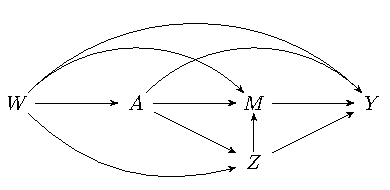
\includegraphics[width=0.8\linewidth]{06-estimation-natural-interventional_files/figure-latex/unnamed-chunk-6-1} 

}

\caption{Directed acyclic graph under intermediate confounders of the mediator-outcome relation affected by treatment}\label{fig:unnamed-chunk-6}
\end{figure}

We define the interventional direct effect as:
\begin{equation*}
  \psi_{\text{PIDE}} = \E(Y_{a^\prime,g_{M \mid a^\star,W}} -
    Y_{a\star,g_{M \mid a^\star,W}}),
\end{equation*}

and the interventional indirect effect as:

\begin{equation*}
  \psi_{\text{PIIE}} = \E(Y_{a^\prime,g_{M \mid a^\prime,W}} -
    Y_{a^\prime,g_{M \mid a^\star,W}}).
\end{equation*}

\hypertarget{simple-case-for-intuition-1}{%
\section{Simple case for intuition}\label{simple-case-for-intuition-1}}

Consider a simple data structure \(O=(W, A, Z, M, Y)\). This SCM is represented in
the above DAG and the following causal models:
\begin{align*}
W & = f_W(U_W)\\
A & = f_A(W, U_A)\\
Z & = f_Z(W, A, U_Z)\\
M & = f_M(W, A, Z, U_M)\\
Y & = f_Y(W, A, Z, M, U_Y),
\end{align*}
where (\(U_W, U_A, U_Z, U_M, U_Y\)) are exogenous random errors. We assume \(A\) is
a single binary treatment, \(Z\) is a single binary intermediate confounder, \(M\)
is a single binary mediator. There are no restrictions on the distribution of
\(W\) or \(Y\).

\(g_{M \mid a^\prime,W}\) represents a stochastic draw from the counterfactual,
conditional distribution of \(M\), as described by
\citet{vanderweele2016mediation}:

\begin{equation*}
  g_{M \mid A,W}(m, a^{\star}, W) \equiv g_{M \mid a^{\star}, W}(W) =
    \sum_{z=0}^1 \P(M=1 \mid Z=z,W) \P(Z=z \mid A=a^{\star}, W).
\end{equation*}

In what follows, we are going to assume that \(g_{M \mid A,W}(m, a^{\star}, W)\)
is known, estimated from observed data, which we call
\(\hat{g}_{M \mid a^{\star}, W}\). This is going to slightly alter the usual
identification assumptions such that we no longer need to assume exchangeability
of \(A\) and the counterfactual \(M\) values. This means the remaining assumptions
are the same as those for controlled direct effects.

\hypertarget{estimation-using-g-computation}{%
\subsection{Estimation using G-Computation}\label{estimation-using-g-computation}}

The estimand \(E(Y_{a^\prime, \hat{g}_{M \mid a^\star,W}})\) can be identified
via sequential regression, which provides the framework for the
G-computation-based estimator. The procedure is as follows

\begin{enumerate}
\def\labelenumi{\arabic{enumi}.}
\tightlist
\item
  Fit a regression of \(Y\) on \(M,Z,W\). Predict outcome values under under
  \(M=m\). We'll call the result \(\bar{Q}_Y(M,Z,W)\).
\item
  Integrate out \(M\) under our stochastic intervention
  \(\hat{g}_{M \mid a^{\star}, W}\). We can do this by evaluating
  \(\E(Y \mid M=m,Z=z,W)\) at each \(m\) and multiplying it by the probability
  that \(M=m\) under \(\hat{g}_{M \mid a^{\star}, W}\), summing over all \(m\).
  We'll call the results \(\bar{Q}^{g}_M(Z,W)\).
\item
  Integrate out \(Z\) and set \(A=a^\prime\). Again, we can do this by evaluating
  the predicted values from Step 2, setting \(A=a^\prime\), and at each \(z\),
  multiplying the prediction by the probability that \(Z=z\) under \(A=a^\prime\).
  We'll call the result \(\bar{Q}^{a^\prime}_Z(W)\).
\item
  Taking the sample mean (marginalizing over \(W\)) gives the parameter
  estimate.
\end{enumerate}

\hypertarget{estimate-with-doubly-robust-methods-based-on-the-eif}{%
\subsection{Estimate with doubly robust methods based on the EIF}\label{estimate-with-doubly-robust-methods-based-on-the-eif}}

The EIF for the parameter \(\Psi(P)(a^{\prime}, \hat{g}_{M \mid a^{\star},W})\),
where, again, \(\hat{g}_{M \mid a^{\star}, W}\) is assumed known, is given by:
\begin{align*}
  D^{\star}(a^{\prime}, \hat{g}_{M \mid a^{\star}, W}) &= \sum_{k=0}^2
      D_k^{\star}(a^{\prime}, \hat{g}_{M \mid a^{\star}, W}), \text{ where }\\
  D^{\star}_0(a^{\prime}, \hat{g}_{M \mid a^{\star}, W}) &=
      \bar{Q}^{a^{\prime}}_{Z(W)} -
      \Psi(P)(a^{\prime}, \hat{g}_{M \mid a^{\star}, W})\\
  D^{\star}_1(a^{\prime}, \hat{g}_{M \mid a^{\star}, W}) &=
      \frac{I(A=a^{\prime})}{\P(A=a^{\prime} \mid W)}(\bar{Q}^{\hat{g}}_M(Z,W)
      - \bar{Q}^{a^{\prime}}_{Z(W)})\\
  D^{\star}_2(a^{\prime}, \hat{g}_{M \mid a^{\star}, W}) &=
      \frac{I(A=a^{\prime})\{I(M=1) \hat{g}_{M \mid a^{\star}, W} +
      I(M=0)(1-\hat{g}_{M \mid a^{\star}, W}) \}}{\P(A=a^{\prime}}
      &\times (Y-\bar{Q}_{Y(M,Z,W)}).
\end{align*}

\hypertarget{estimate-using-tmle}{%
\subsection{Estimate using TMLE}\label{estimate-using-tmle}}

\begin{enumerate}
\def\labelenumi{\arabic{enumi}.}
\tightlist
\item
  We estimate \(g_{Z \mid a^{\star}, W}(W) = \P(Z=1 \mid A=a^{\star}, W)\) from
  a logistic regression of \(Z\) on \(A, W\) setting \(A=a^{\star}\).
\item
  We then estimate \(g_{M \mid z,W}(W) = \P(M=1 \mid Z=z, W)\) from a logistic
  regression of \(M\) on \(Z, W\), setting \(z=\{0,1\}\).
\item
  We use these quantities to calculate \(\hat{g}_{M \mid a^{\star}, W} = \hat{g}_{M \mid z=1,W}\hat{g}_{Z \mid a^{\star}, W} + \hat{g}_{M \mid z=0,W}(1-\hat{g}_{Z|a^{\star}, W})\).
\end{enumerate}

\begin{lstlisting}[language=R]
zmodel <- "z ~ a + w1 "
mmodel <- "m ~ z + w1"
ymodel <- "y ~ m + z*w1"

# make gm and get counterfactual predictions
zfit <- glm(formula = zmodel, family = "binomial", data = obsdat)
mfit <- glm(formula = mmodel, family = "binomial", data = obsdat)

za0 <- predict(zfit,
  newdata = data.frame(w1 = obsdat$w1, a = 0),
  type = "response"
)
za1 <- predict(zfit,
  newdata = data.frame(w1 = obsdat$w1, a = 1),
  type = "response"
)

mz1 <- predict(mfit,
  newdata = data.frame(w1 = obsdat$w1, z = 1),
  type = "response"
)
mz0 < -predict(mfit,
  newdata = data.frame(w1 = obsdat$w1, z = 0),
  type = "response"
)

gm0 <- (mz1 * za0) + (mz0 * (1 - za0))
gma1 <- (mz1 * za1) + (mz0 * (1 - za1))
\end{lstlisting}

\begin{enumerate}
\def\labelenumi{\arabic{enumi}.}
\setcounter{enumi}{3}
\tightlist
\item
  To obtain an estimate of \(\bar{Q}_{Y}(M,Z,W)\), predict values of \(Y\) from a
  regression of \(Y\) on \(M,Z,W\), setting \(m=1\) and \(m=0\), giving
  \(\hat{Y}(m=1, z, w)\) and \(\hat{Y}(m=0, z, w)\).
\end{enumerate}

\begin{lstlisting}[language=R]
tmpdat$qyinit <- cbind(
  predict(glm(
    formula = ymodel, family = "binomial",
    data = data.frame(cbind(datw, z = z, m = m, y = y))
  ),
  newdata = data.frame(cbind(datw, z = z, m = m)), type = "response"
  ),
  predict(glm(
    formula = ymodel, family = "binomial",
    data = data.frame(cbind(datw, z = z, m = m, y = y))
  ),
  newdata = data.frame(cbind(datw, z = z, m = 0)), type = "response"
  ),
  predict(glm(
    formula = ymodel, family = "binomial",
    data = data.frame(cbind(datw, z = z, m = m, y = y))
  ),
  newdata = data.frame(cbind(datw, z = z, m = 1)), type = "response"
  )
)
\end{lstlisting}

\begin{enumerate}
\def\labelenumi{\arabic{enumi}.}
\setcounter{enumi}{4}
\tightlist
\item
  Estimate the weights to be used for the initial targeting step:
  \begin{equation*}
     h_1(a) = \frac{I(A=a)\{I(M=1)\hat{g}_{M \mid a^{\star}, W} +
       I(M=0)(1-\hat{g}_{M \mid a^{\star}, W}) \}}{\P(A=a)\{I(M=1)
       g_{M \mid Z,W} + I(M=0)(1-g_{M \mid Z,W}) \}}
  \end{equation*}
\end{enumerate}

\begin{lstlisting}[language=R]
psa1 <- I(a == 1) / mean(a)
psa0 <- I(a == 0) / mean(1 - a)
mz <- predict(glm(
  formula = mmodel, family = "binomial",
  data = data.frame(cbind(datw, z = z, m = m))
),
newdata = data.frame(cbind(datw, z = z)), type = "response"
)
psm <- (mz * m) + ((1 - mz) * (1 - m))

tmpdat$ha1gma1 <- ((m * gma1 + (1 - m) * (1 - gma1)) / psm) * psa1 * svywt
tmpdat$ha1gma0 <- ((m * gm + (1 - m) * (1 - gm)) / psm) * psa1 * svywt
tmpdat$ha0gma0 <- ((m * gm + (1 - m) * (1 - gm)) / psm) * psa0 * svywt
\end{lstlisting}

\begin{enumerate}
\def\labelenumi{\arabic{enumi}.}
\setcounter{enumi}{5}
\item
  Estimate \(\hat{\epsilon}\) by setting \(\epsilon\) as the intercept of a
  weighted logistic regression model of \(Y\) with
  \(\text{logit}(\hat{\bar{Q}}_{Y}(M,Z,W))\) as an offset and weights
  \(\hat{h}_{1}(a)\). (Note that this is just one possible TMLE.)
\item
  The estimate of \(\bar{Q}_{Y}(M,Z,W)\) is updated by
  \(\hat{\bar{Q}}^{\star}_{Y}(M,Z,W) = \hat{\bar{Q}}_{Y}(\epsilon_n)(M,Z,W)\).
\end{enumerate}

\begin{lstlisting}[language=R]
# for E(Y_{1,gmastar})
epsilonma1g0 <- coef(glm(y ~ 1,
  weights = tmpdat$ha1gma0,
  offset = (qlogis(qyinit[, 1])),
  family = "quasibinomial", data = tmpdat
))
tmpdat$qyupm0a1g0 <- plogis(qlogis(tmpdat$qyinit[, 2]) + epsilonma1g0)
tmpdat$qyupm1a1g0 <- plogis(qlogis(tmpdat$qyinit[, 3]) + epsilonma1g0)

# for E(Y_{1,gma})
epsilonma1g1 <- coef(glm(y ~ 1,
  weights = tmpdat$ha1gma1,
  offset = (qlogis(qyinit[, 1])),
  family = "quasibinomial", data = tmpdat
))
tmpdat$qyupm0a1g1 <- plogis(qlogis(tmpdat$qyinit[, 2]) + epsilonma1g1)
tmpdat$qyupm1a1g1 <- plogis(qlogis(tmpdat$qyinit[, 3]) + epsilonma1g1)

# for E(Y_{0,gmastar})
epsilonma0g0 <- coef(glm(y ~ 1,
  weights = tmpdat$ha0gma0,
  offset = (qlogis(qyinit[, 1])),
  family = "quasibinomial", data = tmpdat
))
tmpdat$qyupm0a0g0 <- plogis(qlogis(tmpdat$qyinit[, 2]) + epsilonma0g0)
tmpdat$qyupm1a0g0 <- plogis(qlogis(tmpdat$qyinit[, 3]) + epsilonma0g0)
\end{lstlisting}

\begin{enumerate}
\def\labelenumi{\arabic{enumi}.}
\setcounter{enumi}{7}
\tightlist
\item
  We next integrate out \(M\) from \(\bar{Q}^{\star}_{Y}(M,Z,W)\). First, we
  estimate \(\bar{Q}^{\star}_{Y,n}(M,Z,W)\) setting \(m=1\) and \(m=0\), giving
  \(\bar{Q}^{\star}_Y(m=1, z, w)\) and \(\bar{Q}^{\star}_Y(m=0, z, w)\). Then,
  multiply these predicted values by their probabilities under
  \(\hat{g}_{M \mid a^{\star},W}(W)\) (for \(a \in \{a, a^{\star}\}\)), and add
  them together (i.e., \(\bar{Q}^{\hat{g}}_{M,n}(Z,W) = \hat{Q}^{\star}_Y(m=1, z, w) \hat{g}_{M|a^{\star},W} + \hat{Q}^{\star}_Y(m=0, z, w)(1-\hat{g}_{M|a^{\star},W})\)).
\end{enumerate}

\begin{lstlisting}[language=R]
tmpdat$Qma1g0 <- tmpdat$qyupm0a1g0 * (1 - gm) + tmpdat$qyupm1a1g0 * gm
tmpdat$Qma1g1 <- tmpdat$qyupm0a1g1 * (1 - gma1) + tmpdat$qyupm1a1g1 * gma1
tmpdat$Qma0g0 <- tmpdat$qyupm0a0g0 * (1 - gm) + tmpdat$qyupm1a0g0 * gm
\end{lstlisting}

\begin{enumerate}
\def\labelenumi{\arabic{enumi}.}
\setcounter{enumi}{8}
\tightlist
\item
  We now fit a regression of \(\bar{Q}^{\hat{g},\star}_{M,n}(Z,W)\) on \(W\)
  among those with \(A=a^\prime\). We call the predicted values from this
  regression \(\hat{\bar{Q}}^{a^\prime}_{Z}(W)\).
\end{enumerate}

\begin{lstlisting}[language=R]
Qzfita1g0 <- glm(
  formula = paste("Qma1g0", qmodel, sep = "~"),
  data = tmpdat[tmpdat$a == 1, ], family = "quasibinomial"
)
Qzfita1g1 <- glm(
  formula = paste("Qma1g1", qmodel, sep = "~"),
  data = tmpdat[tmpdat$a == 1, ], family = "quasibinomial"
)
Qzfita0g0 <- glm(
  formula = paste("Qma0g0", qmodel, sep = "~"),
  data = tmpdat[tmpdat$a == 0, ], family = "quasibinomial"
)

Qza1g0 <- predict(Qzfita1g0, type = "response", newdata = tmpdat)
Qza1g1 <- predict(Qzfita1g1, type = "response", newdata = tmpdat)
Qza0g0 <- predict(Qzfita0g0, type = "response", newdata = tmpdat)
\end{lstlisting}

(Note that if \(A\) were not randomly assigned, we would need to complete a
second targeting step.)

\begin{enumerate}
\def\labelenumi{\arabic{enumi}.}
\setcounter{enumi}{9}
\tightlist
\item
  The empirical mean of these predicted values is the TML estimate of
  \(\Psi(P)(a^\prime, \hat{g}_{M \mid a^{\star}, W})\).
\end{enumerate}

\begin{lstlisting}[language=R]
tmlea1m0 <- sum(Qzupa1g0 * svywt) / sum(svywt)
tmlea1m1 <- sum(Qzupa1g1 * svywt) / sum(svywt)
tmlea0m0 <- sum(Qzupa0g0 * svywt) / sum(svywt)
\end{lstlisting}

\begin{enumerate}
\def\labelenumi{\arabic{enumi}.}
\setcounter{enumi}{10}
\tightlist
\item
  Repeat the above steps for each of the interventions. For example, for
  binary \(A\), we would execute these steps a total of three times to
  estimate:

  \begin{enumerate}
  \def\labelenumii{\arabic{enumii}.}
  \tightlist
  \item
    \(\Psi(P)(1,\hat{g}_{M \mid 1, W})\),
  \item
    \(\Psi(P)(1,\hat{g}_{M \mid 0, W})\), and
  \item
    \(\Psi(P)(0,\hat{g}_{M \mid 0, W})\).
  \end{enumerate}
\item
  The PIDE can then be obtained by substituting estimates of parameters
  \(\Psi(P)(a,\hat{g}_{M \mid a^{\star}, W}) - \Psi(P)(a^{\star},\hat{g}_{M \mid a^{\star}, W})\) and the PIIE
  can be obtained by substituting estimates of parameters
  \(\Psi(P)(a,\hat{g}_{M \mid a,W}) - \Psi(P)(a, \hat{g}_{M \mid a^{\star}, W})\).
\end{enumerate}

\begin{lstlisting}[language=R]
nde <- tmlea1m0 - tmlea0m0
nie <- tmlea1m1 - tmlea1m0
\end{lstlisting}

\begin{enumerate}
\def\labelenumi{\arabic{enumi}.}
\setcounter{enumi}{12}
\tightlist
\item
  The variance can be estimated as the sample variance of the EIF (defined
  above, substituting in the targeted fits) divided by \(n\).
\end{enumerate}

\begin{lstlisting}[language=R]
# first get EIF
tmpdat$qyupa1g0 <- plogis(qlogis(tmpdat$qyinit[, 1]) + epsilonma1g0)
tmpdat$qyupa1g1 <- plogis(qlogis(tmpdat$qyinit[, 1]) + epsilonma1g1)
tmpdat$qyupa0g0 <- plogis(qlogis(tmpdat$qyinit[, 1]) + epsilonma0g0)

eic1a1g0 <- tmpdat$ha1gma0 * (tmpdat$y - tmpdat$qyupa1g0)
eic2a1g0 <- psa1 * svywt * (tmpdat$Qma1g0 - Qzupa1g0)
eic3a1g0 <- Qzupa1g0 - tmlea1m0
eica1g0 <- eic1a1g0 + eic2a1g0 + eic3a1g0

eic1a1g1 <- tmpdat$ha1gma1 * (tmpdat$y - tmpdat$qyupa1g1)
eic2a1g1 <- psa1 * svywt * (tmpdat$Qma1g1 - Qzupa1g1)
eic3a1g1 <- Qzupa1g1 - tmlea1m1
eica1g1 <- eic1a1g1 + eic2a1g1 + eic3a1g1

eic1a0g0 <- tmpdat$ha0gma0 * (tmpdat$y - tmpdat$qyupa0g0)
eic2a0g0 <- psa0 * svywt * (tmpdat$Qma0g0 - Qzupa0g0)
eic3a0g0 <- Qzupa0g0 - tmlea0m0
eica0g0 <- eic1a0g0 + eic2a0g0 + eic3a0g0

# estimands
ndeeic <- eica1g0 - eica0g0
vareic <- var(ndeeic) / nrow(tmpdat)

nieeic <- eica1g1 - eica1g0
varnieeic <- var(nieeic) / nrow(tmpdat)
\end{lstlisting}

\hypertarget{the-general-case}{%
\section{The general case}\label{the-general-case}}

Actually, we would want to have the fixed parameter with the true, unknown
\(g_{M \mid a, W}\) and would like \(M\) to be continuous/multi-dimensional.

This is a pain to do by hand, but Nima made an easy-to-use package for all of us
called \href{https://github.com/nhejazi/medoutcon}{medoutcon}! He will go through
this next.

\hypertarget{estimating-stochastic-effects}{%
\chapter{Estimating stochastic effects}\label{estimating-stochastic-effects}}

{[}TO FILL IN{]}

  \bibliography{book.bib,packages.bib}

\backmatter
\printindex

\end{document}
